%*************************************************************************
% A Classic Thesis Style
% An Homage to The Elements of Typographic Style
%
% Copyright (C) 2017 André Miede and Ivo Pletikosić
%
% If you like the style then I would appreciate a postcard. My address
% can be found in the file ClassicThesis.pdf. A collection of the
% postcards I received so far is available online at
% http://postcards.miede.de
%
% License:
% This program is free software; you can redistribute it and/or modify
% it under the terms of the GNU General Public License as published by
% the Free Software Foundation; either version 2 of the License, or
% (at your option) any later version.
%
% This program is distributed in the hope that it will be useful,
% but WITHOUT ANY WARRANTY; without even the implied warranty of
% MERCHANTABILITY or FITNESS FOR A PARTICULAR PURPOSE.  See the
% GNU General Public License for more details.
%
% You should have received a copy of the GNU General Public License
% along with this program; see the file COPYING.  If not, write to
% the Free Software Foundation, Inc., 59 Temple Place - Suite 330,
% Boston, MA 02111-1307, USA.
%
% PLEASE SEE ALSO THE AUTHORS' NOTE REGARDING THIS LICENSE
% IN THE DOCUMENTATION (ClassicThesis.pdf --> Chapter 1 / Chapter01.tex)
%*************************************************************************
\RequirePackage{silence} % :-\
    \WarningFilter{scrreprt}{Usage of package `titlesec'}
    %\WarningFilter{scrreprt}{Activating an ugly workaround}
    \WarningFilter{titlesec}{Non standard sectioning command detected}
\documentclass[ openright,titlepage,numbers=noenddot,headinclude,%twoside, %1headlines,% letterpaper a4paper
                footinclude=true,cleardoublepage=empty,abstractoff, % <--- obsolete, remove (todo)
                BCOR=5mm,paper=a4,fontsize=11pt,%11pt,a4paper,%
                ngerman,american,%lockflag%
                ]{scrreprt} % change document class to scrartcl to remove chapters


%*************************************************************************
% Note: Make all your adjustments in here
%*************************************************************************
% ****************************************************************************************************
% hdathesis-config.tex 
% Use it at the beginning of your thesis.tex, or as a LaTeX Preamble 
% in your thesis.{tex,lyx} with % ****************************************************************************************************
% hdathesis-config.tex 
% Use it at the beginning of your thesis.tex, or as a LaTeX Preamble 
% in your thesis.{tex,lyx} with % ****************************************************************************************************
% hdathesis-config.tex 
% Use it at the beginning of your thesis.tex, or as a LaTeX Preamble 
% in your thesis.{tex,lyx} with \input{hdathesis-config}
% ****************************************************************************************************

% ****************************************************************************************************
% 1. Personal data and user ad-hoc commands
% ****************************************************************************************************
\newcommand{\myTitle}{Distributed Systems and Algorithms\xspace}
\newcommand{\mySubtitle}{A Summary of the Course  Contents\xspace}
% \newcommand{\myDegree}{Bachelor of Science (B.Sc.)\xspace}
%\newcommand{\myDegree}{Bachelor of Arts (B.A.)\xspace}
%\newcommand{\myDegree}{Master of Science (M.Sc.)\xspace}
%\newcommand{\myDegree}{Master of Arts (M.A.)\xspace}
\newcommand{\myName}{Jonas Weßner\xspace}
\newcommand{\myId}{764805\xspace}
\newcommand{\myProf}{Prof. Dr. Eberhard Max Mühlhäuser }
\newcommand{\myOtherProf}{NO OTHER PROF}
\newcommand{\firstSupervisor}{NO FIRST SUPERVISOR}
\newcommand{\secondSupervisor}{NO SECOND SUPERVISOR}
\newcommand{\myFaculty}{Department of Computer Science\xspace}
\newcommand{\myUni}{Technical University Darmstadt\xspace}
\newcommand{\myLocation}{Darmstadt\xspace}
\newcommand{\myTime}{2. Juni 2022\xspace}
\newcommand{\myVersion}{version 4.4\xspace}

% ****************************************************************************************************
% 2. Is it a master thesis?
% ****************************************************************************************************
%\PassOptionsToPackage{master}{hdahesis} % uncomment if this is a master thesis 

% ****************************************************************************************************
% 3. Does the thesis have a lock flag?
% ****************************************************************************************************
%\PassOptionsToPackage{lockflag}{hdathesis} % uncomment if this thesis has a lock flag 

% ****************************************************************************************************
% 4. Loading some handy packages
% ****************************************************************************************************
% ****************************************************************************************************
% Packages with options that might require adjustments
% ****************************************************************************************************

%\PassOptionsToPackage{ngerman,american}{babel}   % change this to your language(s)
% Spanish languages need extra options in order to work with this template
%\PassOptionsToPackage{spanish,es-lcroman}{babel}
\usepackage{babel}


% ****************************************************************************************************

% ****************************************************************************************************
% 1. Personal data and user ad-hoc commands
% ****************************************************************************************************
\newcommand{\myTitle}{Distributed Systems and Algorithms\xspace}
\newcommand{\mySubtitle}{A Summary of the Course  Contents\xspace}
% \newcommand{\myDegree}{Bachelor of Science (B.Sc.)\xspace}
%\newcommand{\myDegree}{Bachelor of Arts (B.A.)\xspace}
%\newcommand{\myDegree}{Master of Science (M.Sc.)\xspace}
%\newcommand{\myDegree}{Master of Arts (M.A.)\xspace}
\newcommand{\myName}{Jonas Weßner\xspace}
\newcommand{\myId}{764805\xspace}
\newcommand{\myProf}{Prof. Dr. Eberhard Max Mühlhäuser }
\newcommand{\myOtherProf}{NO OTHER PROF}
\newcommand{\firstSupervisor}{NO FIRST SUPERVISOR}
\newcommand{\secondSupervisor}{NO SECOND SUPERVISOR}
\newcommand{\myFaculty}{Department of Computer Science\xspace}
\newcommand{\myUni}{Technical University Darmstadt\xspace}
\newcommand{\myLocation}{Darmstadt\xspace}
\newcommand{\myTime}{2. Juni 2022\xspace}
\newcommand{\myVersion}{version 4.4\xspace}

% ****************************************************************************************************
% 2. Is it a master thesis?
% ****************************************************************************************************
%\PassOptionsToPackage{master}{hdahesis} % uncomment if this is a master thesis 

% ****************************************************************************************************
% 3. Does the thesis have a lock flag?
% ****************************************************************************************************
%\PassOptionsToPackage{lockflag}{hdathesis} % uncomment if this thesis has a lock flag 

% ****************************************************************************************************
% 4. Loading some handy packages
% ****************************************************************************************************
% ****************************************************************************************************
% Packages with options that might require adjustments
% ****************************************************************************************************

%\PassOptionsToPackage{ngerman,american}{babel}   % change this to your language(s)
% Spanish languages need extra options in order to work with this template
%\PassOptionsToPackage{spanish,es-lcroman}{babel}
\usepackage{babel}


% ****************************************************************************************************

% ****************************************************************************************************
% 1. Personal data and user ad-hoc commands
% ****************************************************************************************************
\newcommand{\myTitle}{Distributed Systems and Algorithms\xspace}
\newcommand{\mySubtitle}{A Summary of the Course  Contents\xspace}
% \newcommand{\myDegree}{Bachelor of Science (B.Sc.)\xspace}
%\newcommand{\myDegree}{Bachelor of Arts (B.A.)\xspace}
%\newcommand{\myDegree}{Master of Science (M.Sc.)\xspace}
%\newcommand{\myDegree}{Master of Arts (M.A.)\xspace}
\newcommand{\myName}{Jonas Weßner\xspace}
\newcommand{\myId}{764805\xspace}
\newcommand{\myProf}{Prof. Dr. Eberhard Max Mühlhäuser }
\newcommand{\myOtherProf}{NO OTHER PROF}
\newcommand{\firstSupervisor}{NO FIRST SUPERVISOR}
\newcommand{\secondSupervisor}{NO SECOND SUPERVISOR}
\newcommand{\myFaculty}{Department of Computer Science\xspace}
\newcommand{\myUni}{Technical University Darmstadt\xspace}
\newcommand{\myLocation}{Darmstadt\xspace}
\newcommand{\myTime}{2. Juni 2022\xspace}
\newcommand{\myVersion}{version 4.4\xspace}

% ****************************************************************************************************
% 2. Is it a master thesis?
% ****************************************************************************************************
%\PassOptionsToPackage{master}{hdahesis} % uncomment if this is a master thesis 

% ****************************************************************************************************
% 3. Does the thesis have a lock flag?
% ****************************************************************************************************
%\PassOptionsToPackage{lockflag}{hdathesis} % uncomment if this thesis has a lock flag 

% ****************************************************************************************************
% 4. Loading some handy packages
% ****************************************************************************************************
% ****************************************************************************************************
% Packages with options that might require adjustments
% ****************************************************************************************************

%\PassOptionsToPackage{ngerman,american}{babel}   % change this to your language(s)
% Spanish languages need extra options in order to work with this template
%\PassOptionsToPackage{spanish,es-lcroman}{babel}
\usepackage{babel}


% ****************************************************************************************************
% classicthesis-config.tex
% formerly known as loadpackages.sty, classicthesis-ldpkg.sty, and classicthesis-preamble.sty
% Use it at the beginning of your ClassicThesis.tex, or as a LaTeX Preamble
% in your ClassicThesis.{tex,lyx} with % ****************************************************************************************************
% classicthesis-config.tex
% formerly known as loadpackages.sty, classicthesis-ldpkg.sty, and classicthesis-preamble.sty
% Use it at the beginning of your ClassicThesis.tex, or as a LaTeX Preamble
% in your ClassicThesis.{tex,lyx} with % ****************************************************************************************************
% classicthesis-config.tex
% formerly known as loadpackages.sty, classicthesis-ldpkg.sty, and classicthesis-preamble.sty
% Use it at the beginning of your ClassicThesis.tex, or as a LaTeX Preamble
% in your ClassicThesis.{tex,lyx} with \input{classicthesis-config}
% ****************************************************************************************************
% If you like the classicthesis, then I would appreciate a postcard.
% My address can be found in the file ClassicThesis.pdf. A collection
% of the postcards I received so far is available online at
% http://postcards.miede.de
% ****************************************************************************************************


% ****************************************************************************************************
% 0. Set the encoding of your files. UTF-8 is the only sensible encoding nowadays. If you can't read
% äöüßáéçèê∂åëæƒÏ€ then change the encoding setting in your editor, not the line below. If your editor
% does not support utf8 use another editor!
% ****************************************************************************************************
\PassOptionsToPackage{utf8}{inputenc}
\usepackage{inputenc}

% ****************************************************************************************************
% 1. Configure classicthesis for your needs here, e.g., remove "drafting" below
% in order to deactivate the time-stamp on the pages
% (see ClassicThesis.pdf for more information):
% ****************************************************************************************************
\PassOptionsToPackage{
  drafting=false,   % print version information on the bottom of the pages
  tocaligned=false, % the left column of the toc will be aligned (no indentation)
  dottedtoc=true,   % page numbers in ToC flushed right
  parts=true,       % use part division
  eulerchapternumbers=true, % use AMS Euler for chapter font (otherwise Palatino)
  linedheaders=false,       % chaper headers will have line above and beneath
  floatperchapter=true,     % numbering per chapter for all floats (i.e., Figure 1.1)
  listings=true,    % load listings package and setup LoL
  subfig=true,      % setup for preloaded subfig package
  eulermath=false,  % use awesome Euler fonts for mathematical formulae (only with pdfLaTeX)
  beramono=true,    % toggle a nice monospaced font (w/ bold)
  minionpro=false   % setup for minion pro font; use minion pro small caps as well (only with pdfLaTeX)
}{classicthesis}


% ****************************************************************************************************
% 2. Personal data and user ad-hoc commands
% ****************************************************************************************************
%\newcommand{\myTitle}{A Classic Thesis Style\xspace}
%\newcommand{\mySubtitle}{An Homage to The Elements of Typographic Style\xspace}
%\newcommand{\myDegree}{Doktor-Ingenieur (Dr.-Ing.)\xspace}
%\newcommand{\myName}{André Miede\xspace}
%\newcommand{\myProf}{Put name here\xspace}
%\newcommand{\myOtherProf}{Put name here\xspace}
%\newcommand{\mySupervisor}{Put name here\xspace}
%\newcommand{\myFaculty}{Put data here\xspace}
%\newcommand{\myDepartment}{Put data here\xspace}
%\newcommand{\myUni}{Put data here\xspace}
%\newcommand{\myLocation}{Saarbrücken\xspace}
%\newcommand{\myTime}{October 2017\xspace}
%\newcommand{\myVersion}{version 4.4}

% ********************************************************************
% Setup, finetuning, and useful commands
% ********************************************************************
\newcounter{dummy} % necessary for correct hyperlinks (to index, bib, etc.)
\newlength{\abcd} % for ab..z string length calculation
\providecommand{\mLyX}{L\kern-.1667em\lower.25em\hbox{Y}\kern-.125emX\@}
\newcommand{\ie}{i.\,e.}
\newcommand{\Ie}{I.\,e.}
\newcommand{\eg}{e.\,g.}
\newcommand{\Eg}{E.\,g.}
% ****************************************************************************************************


% ****************************************************************************************************
% 3. Loading some handy packages
% ****************************************************************************************************
% ********************************************************************
% Packages with options that might require adjustments
% ********************************************************************
%\PassOptionsToPackage{ngerman,american}{babel}   % change this to your language(s), main language last
% Spanish languages need extra options in order to work with this template
%\PassOptionsToPackage{spanish,es-lcroman}{babel}
\usepackage{babel}

\usepackage{csquotes}

\PassOptionsToPackage{%
  %backend=biber,bibencoding=utf8, %instead of bibtex
  backend=bibtex8,bibencoding=ascii,%
  language=auto,%
  style=numeric-comp,%
  %style=alphabetic,%
  %style=authoryear-comp, % Author 1999, 2010
  %bibstyle=authoryear,dashed=false, % dashed: substitute rep. author with ---
  sorting=nyt, % name, year, title
  maxbibnames=10, % default: 3, et al.
  %backref=true,%
  natbib=true % natbib compatibility mode (\citep and \citet still work)
}{biblatex}
\usepackage{biblatex}

\PassOptionsToPackage{fleqn}{amsmath}       % math environments and more by the AMS
\usepackage{amsmath}

\PassOptionsToPackage{doublespacing}{hdathesis}  % options: abbrev exam big wiwi english master
\usepackage{hdathesis}

% ********************************************************************
% General useful packages
% ********************************************************************
\PassOptionsToPackage{T1}{fontenc} % T2A for cyrillics
\usepackage{fontenc}
\usepackage{textcomp} % fix warning with missing font shapes
\usepackage{scrhack} % fix warnings when using KOMA with listings package
\usepackage{xspace} % to get the spacing after macros right
\usepackage{mparhack} % get marginpar right
%\usepackage{fixltx2e} % fixes some LaTeX stuff --> since 2015 in the LaTeX kernel (see below)
% \usepackage[latest]{latexrelease} % emulate newer kernel version if older is detected
\PassOptionsToPackage{printonlyused,smaller}{acronym}
\usepackage{acronym} % nice macros for handling all acronyms in the thesis
%\renewcommand{\bflabel}[1]{{#1}\hfill} % fix the list of acronyms --> no longer working
%\renewcommand*{\acsfont}[1]{\textsc{#1}}
%\renewcommand*{\aclabelfont}[1]{\acsfont{#1}}
%\def\bflabel#1{{#1\hfill}}
\def\bflabel#1{{\acsfont{#1}\hfill}}
\def\aclabelfont#1{\acsfont{#1}}
% ****************************************************************************************************
%\usepackage{pgfplots} % External TikZ/PGF support (thanks to Andreas Nautsch)
%\usetikzlibrary{external}
%\tikzexternalize[mode=list and make, prefix=ext-tikz/]
% ****************************************************************************************************


% ****************************************************************************************************
% 4. Setup floats: tables, (sub)figures, and captions
% ****************************************************************************************************
\usepackage{tabularx} % better tables
\setlength{\extrarowheight}{3pt} % increase table row height
\newcommand{\tableheadline}[1]{\multicolumn{1}{c}{\spacedlowsmallcaps{#1}}}
\newcommand{\myfloatalign}{\centering} % to be used with each float for alignment
\usepackage{caption}
% Thanks to cgnieder and Claus Lahiri
% http://tex.stackexchange.com/questions/69349/spacedlowsmallcaps-in-caption-label
% [REMOVED DUE TO OTHER PROBLEMS, SEE ISSUE #82]
%\DeclareCaptionLabelFormat{smallcaps}{\bothIfFirst{#1}{~}\MakeTextLowercase{\textsc{#2}}}
%\captionsetup{font=small,labelformat=smallcaps} % format=hang,
\captionsetup{font=small} % format=hang,
\usepackage{subfig}
% ****************************************************************************************************


% ****************************************************************************************************
% 5. Setup code listings
% ****************************************************************************************************
\usepackage{listings}
%\lstset{emph={trueIndex,root},emphstyle=\color{BlueViolet}}%\underbar} % for special keywords
\lstset{language=[LaTeX]Tex,%C++,
  morekeywords={PassOptionsToPackage,selectlanguage},
  keywordstyle=\color{RoyalBlue},%\bfseries,
  basicstyle=\small\ttfamily,
  %identifierstyle=\color{NavyBlue},
  commentstyle=\color{Green}\ttfamily,
  stringstyle=\rmfamily,
  numbers=none,%left,%
  numberstyle=\scriptsize,%\tiny
  stepnumber=5,
  numbersep=8pt,
  showstringspaces=false,
  breaklines=true,
  %frameround=ftff,
  %frame=single,
  belowcaptionskip=.75\baselineskip
  %frame=L
}
% ****************************************************************************************************


% ****************************************************************************************************
% 6. PDFLaTeX, hyperreferences, and citation backreferences
% ****************************************************************************************************
% ********************************************************************
% Using PDFLaTeX
% ********************************************************************
\PassOptionsToPackage{hyperfootnotes=false,pdfpagelabels}{hyperref}
\usepackage{hyperref}  % backref linktocpage pagebackref
%\ifpdf
%\pdfcompresslevel=9
%\pdfadjustspacing=1
%\fi
%\PassOptionsToPackage{pdftex}{graphicx} %%%IVO: driver will be chosen automatically
\usepackage{graphicx}


% ********************************************************************
% Hyperreferences
% ********************************************************************
\hypersetup{%
  %draft, % hyperref's draft mode, for printing see below
  colorlinks=true, linktocpage=true, pdfstartpage=3, pdfstartview=FitV,%
  % uncomment the following line if you want to have black links (e.g., for printing)
  %colorlinks=false, linktocpage=false, pdfstartpage=3, pdfstartview=FitV, pdfborder={0 0 0},%
  breaklinks=true, pdfpagemode=UseNone, pageanchor=true, pdfpagemode=UseOutlines,%
  plainpages=false, bookmarksnumbered, bookmarksopen=true, bookmarksopenlevel=1,%
  hypertexnames=true, pdfhighlight=/O,%nesting=true,%frenchlinks,%
  urlcolor=webbrown, linkcolor=RoyalBlue, citecolor=webgreen, %pagecolor=RoyalBlue,%
  %urlcolor=Black, linkcolor=Black, citecolor=Black, %pagecolor=Black,%
  pdftitle={\myTitle},%
  pdfauthor={\textcopyright\ \myName, \myUni, \myFaculty},%
  pdfsubject={},%
  pdfkeywords={},%
  pdfcreator={pdfLaTeX},%
  pdfproducer={LaTeX with hyperref and classicthesis}%
}

% ********************************************************************
% Setup autoreferences
% ********************************************************************
% There are some issues regarding autorefnames
% http://www.ureader.de/msg/136221647.aspx
% http://www.tex.ac.uk/cgi-bin/texfaq2html?label=latexwords
% you have to redefine the makros for the
% language you use, e.g., american, ngerman
% (as chosen when loading babel/AtBeginDocument)
% ********************************************************************
\makeatletter
\@ifpackageloaded{babel}%
{%
  \addto\extrasamerican{%
    \renewcommand*{\figureautorefname}{Figure}%
    \renewcommand*{\tableautorefname}{Table}%
    \renewcommand*{\partautorefname}{Part}%
    \renewcommand*{\chapterautorefname}{Chapter}%
    \renewcommand*{\sectionautorefname}{Section}%
    \renewcommand*{\subsectionautorefname}{Section}%
    \renewcommand*{\subsubsectionautorefname}{Section}%
  }%
  \addto\extrasngerman{%
    \renewcommand*{\paragraphautorefname}{Absatz}%
    \renewcommand*{\subparagraphautorefname}{Unterabsatz}%
    \renewcommand*{\footnoteautorefname}{Fu\"snote}%
    \renewcommand*{\FancyVerbLineautorefname}{Zeile}%
    \renewcommand*{\theoremautorefname}{Theorem}%
    \renewcommand*{\appendixautorefname}{Anhang}%
    \renewcommand*{\equationautorefname}{Gleichung}%
    \renewcommand*{\itemautorefname}{Punkt}%
  }%
  % Fix to getting autorefs for subfigures right (thanks to Belinda Vogt for changing the definition)
  \providecommand{\subfigureautorefname}{\figureautorefname}%
}{\relax}
\makeatother


% ****************************************************************************************************
% 7. Last calls before the bar closes
% ****************************************************************************************************
% ********************************************************************
% Development Stuff
% ********************************************************************
\listfiles
%\PassOptionsToPackage{l2tabu,orthodox,abort}{nag}
%  \usepackage{nag}
%\PassOptionsToPackage{warning, all}{onlyamsmath}
%  \usepackage{onlyamsmath}

% ********************************************************************
% Last, but not least...
% ********************************************************************
\usepackage{classicthesis}
% ****************************************************************************************************


% ****************************************************************************************************
% 8. Further adjustments (experimental)
% ****************************************************************************************************
% ********************************************************************
% Changing the text area
% ********************************************************************
%\areaset[current]{312pt}{761pt} % 686 (factor 2.2) + 33 head + 42 head \the\footskip
%\setlength{\marginparwidth}{7em}%
%\setlength{\marginparsep}{2em}%

% ********************************************************************
% Using different fonts
% ********************************************************************
%\usepackage[oldstylenums]{kpfonts} % oldstyle notextcomp
%\usepackage[osf]{libertine}
%\usepackage[light,condensed,math]{iwona}
%\renewcommand{\sfdefault}{iwona}
%\usepackage{lmodern} % <-- no osf support :-(
%\usepackage{cfr-lm} %
%\usepackage[urw-garamond]{mathdesign} <-- no osf support :-(
%\usepackage[default,osfigures]{opensans} % scale=0.95
%\usepackage[sfdefault]{FiraSans}
% ********************************************************************
% \usepackage[largesc,osf]{newpxtext}
% Used to fix these:
% https://bitbucket.org/amiede/classicthesis/issues/139/italics-in-pallatino-capitals-chapter
% https://bitbucket.org/amiede/classicthesis/issues/45/problema-testatine-su-classicthesis-style
% ********************************************************************
%\linespread{1.05} % a bit more for Palatino
% ****************************************************************************************************

% used for referencing single items of an "enumerate"-list
\usepackage{enumitem}


% paragraph style: {indentation}{spacing}{white space at right side of last word in paragraph}
\newcommand\customparskip{0.5\baselineskip} % define custom parameter skip
\newcommand\noskip{\vspace{-\customparskip}} % create command to revert custom parameter skip for one paragraph
\setparsizes{0pt}{\customparskip}{0pt plus 1fil} % set paragraph sizes for the entire document

% special math functionality
\usepackage{mathtools}

\usepackage{float}
\usepackage{wrapfig}
% ****************************************************************************************************
% If you like the classicthesis, then I would appreciate a postcard.
% My address can be found in the file ClassicThesis.pdf. A collection
% of the postcards I received so far is available online at
% http://postcards.miede.de
% ****************************************************************************************************


% ****************************************************************************************************
% 0. Set the encoding of your files. UTF-8 is the only sensible encoding nowadays. If you can't read
% äöüßáéçèê∂åëæƒÏ€ then change the encoding setting in your editor, not the line below. If your editor
% does not support utf8 use another editor!
% ****************************************************************************************************
\PassOptionsToPackage{utf8}{inputenc}
\usepackage{inputenc}

% ****************************************************************************************************
% 1. Configure classicthesis for your needs here, e.g., remove "drafting" below
% in order to deactivate the time-stamp on the pages
% (see ClassicThesis.pdf for more information):
% ****************************************************************************************************
\PassOptionsToPackage{
  drafting=false,   % print version information on the bottom of the pages
  tocaligned=false, % the left column of the toc will be aligned (no indentation)
  dottedtoc=true,   % page numbers in ToC flushed right
  parts=true,       % use part division
  eulerchapternumbers=true, % use AMS Euler for chapter font (otherwise Palatino)
  linedheaders=false,       % chaper headers will have line above and beneath
  floatperchapter=true,     % numbering per chapter for all floats (i.e., Figure 1.1)
  listings=true,    % load listings package and setup LoL
  subfig=true,      % setup for preloaded subfig package
  eulermath=false,  % use awesome Euler fonts for mathematical formulae (only with pdfLaTeX)
  beramono=true,    % toggle a nice monospaced font (w/ bold)
  minionpro=false   % setup for minion pro font; use minion pro small caps as well (only with pdfLaTeX)
}{classicthesis}


% ****************************************************************************************************
% 2. Personal data and user ad-hoc commands
% ****************************************************************************************************
%\newcommand{\myTitle}{A Classic Thesis Style\xspace}
%\newcommand{\mySubtitle}{An Homage to The Elements of Typographic Style\xspace}
%\newcommand{\myDegree}{Doktor-Ingenieur (Dr.-Ing.)\xspace}
%\newcommand{\myName}{André Miede\xspace}
%\newcommand{\myProf}{Put name here\xspace}
%\newcommand{\myOtherProf}{Put name here\xspace}
%\newcommand{\mySupervisor}{Put name here\xspace}
%\newcommand{\myFaculty}{Put data here\xspace}
%\newcommand{\myDepartment}{Put data here\xspace}
%\newcommand{\myUni}{Put data here\xspace}
%\newcommand{\myLocation}{Saarbrücken\xspace}
%\newcommand{\myTime}{October 2017\xspace}
%\newcommand{\myVersion}{version 4.4}

% ********************************************************************
% Setup, finetuning, and useful commands
% ********************************************************************
\newcounter{dummy} % necessary for correct hyperlinks (to index, bib, etc.)
\newlength{\abcd} % for ab..z string length calculation
\providecommand{\mLyX}{L\kern-.1667em\lower.25em\hbox{Y}\kern-.125emX\@}
\newcommand{\ie}{i.\,e.}
\newcommand{\Ie}{I.\,e.}
\newcommand{\eg}{e.\,g.}
\newcommand{\Eg}{E.\,g.}
% ****************************************************************************************************


% ****************************************************************************************************
% 3. Loading some handy packages
% ****************************************************************************************************
% ********************************************************************
% Packages with options that might require adjustments
% ********************************************************************
%\PassOptionsToPackage{ngerman,american}{babel}   % change this to your language(s), main language last
% Spanish languages need extra options in order to work with this template
%\PassOptionsToPackage{spanish,es-lcroman}{babel}
\usepackage{babel}

\usepackage{csquotes}

\PassOptionsToPackage{%
  %backend=biber,bibencoding=utf8, %instead of bibtex
  backend=bibtex8,bibencoding=ascii,%
  language=auto,%
  style=numeric-comp,%
  %style=alphabetic,%
  %style=authoryear-comp, % Author 1999, 2010
  %bibstyle=authoryear,dashed=false, % dashed: substitute rep. author with ---
  sorting=nyt, % name, year, title
  maxbibnames=10, % default: 3, et al.
  %backref=true,%
  natbib=true % natbib compatibility mode (\citep and \citet still work)
}{biblatex}
\usepackage{biblatex}

\PassOptionsToPackage{fleqn}{amsmath}       % math environments and more by the AMS
\usepackage{amsmath}

\PassOptionsToPackage{doublespacing}{hdathesis}  % options: abbrev exam big wiwi english master
\usepackage{hdathesis}

% ********************************************************************
% General useful packages
% ********************************************************************
\PassOptionsToPackage{T1}{fontenc} % T2A for cyrillics
\usepackage{fontenc}
\usepackage{textcomp} % fix warning with missing font shapes
\usepackage{scrhack} % fix warnings when using KOMA with listings package
\usepackage{xspace} % to get the spacing after macros right
\usepackage{mparhack} % get marginpar right
%\usepackage{fixltx2e} % fixes some LaTeX stuff --> since 2015 in the LaTeX kernel (see below)
% \usepackage[latest]{latexrelease} % emulate newer kernel version if older is detected
\PassOptionsToPackage{printonlyused,smaller}{acronym}
\usepackage{acronym} % nice macros for handling all acronyms in the thesis
%\renewcommand{\bflabel}[1]{{#1}\hfill} % fix the list of acronyms --> no longer working
%\renewcommand*{\acsfont}[1]{\textsc{#1}}
%\renewcommand*{\aclabelfont}[1]{\acsfont{#1}}
%\def\bflabel#1{{#1\hfill}}
\def\bflabel#1{{\acsfont{#1}\hfill}}
\def\aclabelfont#1{\acsfont{#1}}
% ****************************************************************************************************
%\usepackage{pgfplots} % External TikZ/PGF support (thanks to Andreas Nautsch)
%\usetikzlibrary{external}
%\tikzexternalize[mode=list and make, prefix=ext-tikz/]
% ****************************************************************************************************


% ****************************************************************************************************
% 4. Setup floats: tables, (sub)figures, and captions
% ****************************************************************************************************
\usepackage{tabularx} % better tables
\setlength{\extrarowheight}{3pt} % increase table row height
\newcommand{\tableheadline}[1]{\multicolumn{1}{c}{\spacedlowsmallcaps{#1}}}
\newcommand{\myfloatalign}{\centering} % to be used with each float for alignment
\usepackage{caption}
% Thanks to cgnieder and Claus Lahiri
% http://tex.stackexchange.com/questions/69349/spacedlowsmallcaps-in-caption-label
% [REMOVED DUE TO OTHER PROBLEMS, SEE ISSUE #82]
%\DeclareCaptionLabelFormat{smallcaps}{\bothIfFirst{#1}{~}\MakeTextLowercase{\textsc{#2}}}
%\captionsetup{font=small,labelformat=smallcaps} % format=hang,
\captionsetup{font=small} % format=hang,
\usepackage{subfig}
% ****************************************************************************************************


% ****************************************************************************************************
% 5. Setup code listings
% ****************************************************************************************************
\usepackage{listings}
%\lstset{emph={trueIndex,root},emphstyle=\color{BlueViolet}}%\underbar} % for special keywords
\lstset{language=[LaTeX]Tex,%C++,
  morekeywords={PassOptionsToPackage,selectlanguage},
  keywordstyle=\color{RoyalBlue},%\bfseries,
  basicstyle=\small\ttfamily,
  %identifierstyle=\color{NavyBlue},
  commentstyle=\color{Green}\ttfamily,
  stringstyle=\rmfamily,
  numbers=none,%left,%
  numberstyle=\scriptsize,%\tiny
  stepnumber=5,
  numbersep=8pt,
  showstringspaces=false,
  breaklines=true,
  %frameround=ftff,
  %frame=single,
  belowcaptionskip=.75\baselineskip
  %frame=L
}
% ****************************************************************************************************


% ****************************************************************************************************
% 6. PDFLaTeX, hyperreferences, and citation backreferences
% ****************************************************************************************************
% ********************************************************************
% Using PDFLaTeX
% ********************************************************************
\PassOptionsToPackage{hyperfootnotes=false,pdfpagelabels}{hyperref}
\usepackage{hyperref}  % backref linktocpage pagebackref
%\ifpdf
%\pdfcompresslevel=9
%\pdfadjustspacing=1
%\fi
%\PassOptionsToPackage{pdftex}{graphicx} %%%IVO: driver will be chosen automatically
\usepackage{graphicx}


% ********************************************************************
% Hyperreferences
% ********************************************************************
\hypersetup{%
  %draft, % hyperref's draft mode, for printing see below
  colorlinks=true, linktocpage=true, pdfstartpage=3, pdfstartview=FitV,%
  % uncomment the following line if you want to have black links (e.g., for printing)
  %colorlinks=false, linktocpage=false, pdfstartpage=3, pdfstartview=FitV, pdfborder={0 0 0},%
  breaklinks=true, pdfpagemode=UseNone, pageanchor=true, pdfpagemode=UseOutlines,%
  plainpages=false, bookmarksnumbered, bookmarksopen=true, bookmarksopenlevel=1,%
  hypertexnames=true, pdfhighlight=/O,%nesting=true,%frenchlinks,%
  urlcolor=webbrown, linkcolor=RoyalBlue, citecolor=webgreen, %pagecolor=RoyalBlue,%
  %urlcolor=Black, linkcolor=Black, citecolor=Black, %pagecolor=Black,%
  pdftitle={\myTitle},%
  pdfauthor={\textcopyright\ \myName, \myUni, \myFaculty},%
  pdfsubject={},%
  pdfkeywords={},%
  pdfcreator={pdfLaTeX},%
  pdfproducer={LaTeX with hyperref and classicthesis}%
}

% ********************************************************************
% Setup autoreferences
% ********************************************************************
% There are some issues regarding autorefnames
% http://www.ureader.de/msg/136221647.aspx
% http://www.tex.ac.uk/cgi-bin/texfaq2html?label=latexwords
% you have to redefine the makros for the
% language you use, e.g., american, ngerman
% (as chosen when loading babel/AtBeginDocument)
% ********************************************************************
\makeatletter
\@ifpackageloaded{babel}%
{%
  \addto\extrasamerican{%
    \renewcommand*{\figureautorefname}{Figure}%
    \renewcommand*{\tableautorefname}{Table}%
    \renewcommand*{\partautorefname}{Part}%
    \renewcommand*{\chapterautorefname}{Chapter}%
    \renewcommand*{\sectionautorefname}{Section}%
    \renewcommand*{\subsectionautorefname}{Section}%
    \renewcommand*{\subsubsectionautorefname}{Section}%
  }%
  \addto\extrasngerman{%
    \renewcommand*{\paragraphautorefname}{Absatz}%
    \renewcommand*{\subparagraphautorefname}{Unterabsatz}%
    \renewcommand*{\footnoteautorefname}{Fu\"snote}%
    \renewcommand*{\FancyVerbLineautorefname}{Zeile}%
    \renewcommand*{\theoremautorefname}{Theorem}%
    \renewcommand*{\appendixautorefname}{Anhang}%
    \renewcommand*{\equationautorefname}{Gleichung}%
    \renewcommand*{\itemautorefname}{Punkt}%
  }%
  % Fix to getting autorefs for subfigures right (thanks to Belinda Vogt for changing the definition)
  \providecommand{\subfigureautorefname}{\figureautorefname}%
}{\relax}
\makeatother


% ****************************************************************************************************
% 7. Last calls before the bar closes
% ****************************************************************************************************
% ********************************************************************
% Development Stuff
% ********************************************************************
\listfiles
%\PassOptionsToPackage{l2tabu,orthodox,abort}{nag}
%  \usepackage{nag}
%\PassOptionsToPackage{warning, all}{onlyamsmath}
%  \usepackage{onlyamsmath}

% ********************************************************************
% Last, but not least...
% ********************************************************************
\usepackage{classicthesis}
% ****************************************************************************************************


% ****************************************************************************************************
% 8. Further adjustments (experimental)
% ****************************************************************************************************
% ********************************************************************
% Changing the text area
% ********************************************************************
%\areaset[current]{312pt}{761pt} % 686 (factor 2.2) + 33 head + 42 head \the\footskip
%\setlength{\marginparwidth}{7em}%
%\setlength{\marginparsep}{2em}%

% ********************************************************************
% Using different fonts
% ********************************************************************
%\usepackage[oldstylenums]{kpfonts} % oldstyle notextcomp
%\usepackage[osf]{libertine}
%\usepackage[light,condensed,math]{iwona}
%\renewcommand{\sfdefault}{iwona}
%\usepackage{lmodern} % <-- no osf support :-(
%\usepackage{cfr-lm} %
%\usepackage[urw-garamond]{mathdesign} <-- no osf support :-(
%\usepackage[default,osfigures]{opensans} % scale=0.95
%\usepackage[sfdefault]{FiraSans}
% ********************************************************************
% \usepackage[largesc,osf]{newpxtext}
% Used to fix these:
% https://bitbucket.org/amiede/classicthesis/issues/139/italics-in-pallatino-capitals-chapter
% https://bitbucket.org/amiede/classicthesis/issues/45/problema-testatine-su-classicthesis-style
% ********************************************************************
%\linespread{1.05} % a bit more for Palatino
% ****************************************************************************************************

% used for referencing single items of an "enumerate"-list
\usepackage{enumitem}


% paragraph style: {indentation}{spacing}{white space at right side of last word in paragraph}
\newcommand\customparskip{0.5\baselineskip} % define custom parameter skip
\newcommand\noskip{\vspace{-\customparskip}} % create command to revert custom parameter skip for one paragraph
\setparsizes{0pt}{\customparskip}{0pt plus 1fil} % set paragraph sizes for the entire document

% special math functionality
\usepackage{mathtools}

\usepackage{float}
\usepackage{wrapfig}
% ****************************************************************************************************
% If you like the classicthesis, then I would appreciate a postcard.
% My address can be found in the file ClassicThesis.pdf. A collection
% of the postcards I received so far is available online at
% http://postcards.miede.de
% ****************************************************************************************************


% ****************************************************************************************************
% 0. Set the encoding of your files. UTF-8 is the only sensible encoding nowadays. If you can't read
% äöüßáéçèê∂åëæƒÏ€ then change the encoding setting in your editor, not the line below. If your editor
% does not support utf8 use another editor!
% ****************************************************************************************************
\PassOptionsToPackage{utf8}{inputenc}
\usepackage{inputenc}

% ****************************************************************************************************
% 1. Configure classicthesis for your needs here, e.g., remove "drafting" below
% in order to deactivate the time-stamp on the pages
% (see ClassicThesis.pdf for more information):
% ****************************************************************************************************
\PassOptionsToPackage{
  drafting=false,   % print version information on the bottom of the pages
  tocaligned=false, % the left column of the toc will be aligned (no indentation)
  dottedtoc=true,   % page numbers in ToC flushed right
  parts=true,       % use part division
  eulerchapternumbers=true, % use AMS Euler for chapter font (otherwise Palatino)
  linedheaders=false,       % chaper headers will have line above and beneath
  floatperchapter=true,     % numbering per chapter for all floats (i.e., Figure 1.1)
  listings=true,    % load listings package and setup LoL
  subfig=true,      % setup for preloaded subfig package
  eulermath=false,  % use awesome Euler fonts for mathematical formulae (only with pdfLaTeX)
  beramono=true,    % toggle a nice monospaced font (w/ bold)
  minionpro=false   % setup for minion pro font; use minion pro small caps as well (only with pdfLaTeX)
}{classicthesis}


% ****************************************************************************************************
% 2. Personal data and user ad-hoc commands
% ****************************************************************************************************
%\newcommand{\myTitle}{A Classic Thesis Style\xspace}
%\newcommand{\mySubtitle}{An Homage to The Elements of Typographic Style\xspace}
%\newcommand{\myDegree}{Doktor-Ingenieur (Dr.-Ing.)\xspace}
%\newcommand{\myName}{André Miede\xspace}
%\newcommand{\myProf}{Put name here\xspace}
%\newcommand{\myOtherProf}{Put name here\xspace}
%\newcommand{\mySupervisor}{Put name here\xspace}
%\newcommand{\myFaculty}{Put data here\xspace}
%\newcommand{\myDepartment}{Put data here\xspace}
%\newcommand{\myUni}{Put data here\xspace}
%\newcommand{\myLocation}{Saarbrücken\xspace}
%\newcommand{\myTime}{October 2017\xspace}
%\newcommand{\myVersion}{version 4.4}

% ********************************************************************
% Setup, finetuning, and useful commands
% ********************************************************************
\newcounter{dummy} % necessary for correct hyperlinks (to index, bib, etc.)
\newlength{\abcd} % for ab..z string length calculation
\providecommand{\mLyX}{L\kern-.1667em\lower.25em\hbox{Y}\kern-.125emX\@}
\newcommand{\ie}{i.\,e.}
\newcommand{\Ie}{I.\,e.}
\newcommand{\eg}{e.\,g.}
\newcommand{\Eg}{E.\,g.}
% ****************************************************************************************************


% ****************************************************************************************************
% 3. Loading some handy packages
% ****************************************************************************************************
% ********************************************************************
% Packages with options that might require adjustments
% ********************************************************************
%\PassOptionsToPackage{ngerman,american}{babel}   % change this to your language(s), main language last
% Spanish languages need extra options in order to work with this template
%\PassOptionsToPackage{spanish,es-lcroman}{babel}
\usepackage{babel}

\usepackage{csquotes}

\PassOptionsToPackage{%
  %backend=biber,bibencoding=utf8, %instead of bibtex
  backend=bibtex8,bibencoding=ascii,%
  language=auto,%
  style=numeric-comp,%
  %style=alphabetic,%
  %style=authoryear-comp, % Author 1999, 2010
  %bibstyle=authoryear,dashed=false, % dashed: substitute rep. author with ---
  sorting=nyt, % name, year, title
  maxbibnames=10, % default: 3, et al.
  %backref=true,%
  natbib=true % natbib compatibility mode (\citep and \citet still work)
}{biblatex}
\usepackage{biblatex}

\PassOptionsToPackage{fleqn}{amsmath}       % math environments and more by the AMS
\usepackage{amsmath}

\PassOptionsToPackage{doublespacing}{hdathesis}  % options: abbrev exam big wiwi english master
\usepackage{hdathesis}

% ********************************************************************
% General useful packages
% ********************************************************************
\PassOptionsToPackage{T1}{fontenc} % T2A for cyrillics
\usepackage{fontenc}
\usepackage{textcomp} % fix warning with missing font shapes
\usepackage{scrhack} % fix warnings when using KOMA with listings package
\usepackage{xspace} % to get the spacing after macros right
\usepackage{mparhack} % get marginpar right
%\usepackage{fixltx2e} % fixes some LaTeX stuff --> since 2015 in the LaTeX kernel (see below)
% \usepackage[latest]{latexrelease} % emulate newer kernel version if older is detected
\PassOptionsToPackage{printonlyused,smaller}{acronym}
\usepackage{acronym} % nice macros for handling all acronyms in the thesis
%\renewcommand{\bflabel}[1]{{#1}\hfill} % fix the list of acronyms --> no longer working
%\renewcommand*{\acsfont}[1]{\textsc{#1}}
%\renewcommand*{\aclabelfont}[1]{\acsfont{#1}}
%\def\bflabel#1{{#1\hfill}}
\def\bflabel#1{{\acsfont{#1}\hfill}}
\def\aclabelfont#1{\acsfont{#1}}
% ****************************************************************************************************
%\usepackage{pgfplots} % External TikZ/PGF support (thanks to Andreas Nautsch)
%\usetikzlibrary{external}
%\tikzexternalize[mode=list and make, prefix=ext-tikz/]
% ****************************************************************************************************


% ****************************************************************************************************
% 4. Setup floats: tables, (sub)figures, and captions
% ****************************************************************************************************
\usepackage{tabularx} % better tables
\setlength{\extrarowheight}{3pt} % increase table row height
\newcommand{\tableheadline}[1]{\multicolumn{1}{c}{\spacedlowsmallcaps{#1}}}
\newcommand{\myfloatalign}{\centering} % to be used with each float for alignment
\usepackage{caption}
% Thanks to cgnieder and Claus Lahiri
% http://tex.stackexchange.com/questions/69349/spacedlowsmallcaps-in-caption-label
% [REMOVED DUE TO OTHER PROBLEMS, SEE ISSUE #82]
%\DeclareCaptionLabelFormat{smallcaps}{\bothIfFirst{#1}{~}\MakeTextLowercase{\textsc{#2}}}
%\captionsetup{font=small,labelformat=smallcaps} % format=hang,
\captionsetup{font=small} % format=hang,
\usepackage{subfig}
% ****************************************************************************************************


% ****************************************************************************************************
% 5. Setup code listings
% ****************************************************************************************************
\usepackage{listings}
%\lstset{emph={trueIndex,root},emphstyle=\color{BlueViolet}}%\underbar} % for special keywords
\lstset{language=[LaTeX]Tex,%C++,
  morekeywords={PassOptionsToPackage,selectlanguage},
  keywordstyle=\color{RoyalBlue},%\bfseries,
  basicstyle=\small\ttfamily,
  %identifierstyle=\color{NavyBlue},
  commentstyle=\color{Green}\ttfamily,
  stringstyle=\rmfamily,
  numbers=none,%left,%
  numberstyle=\scriptsize,%\tiny
  stepnumber=5,
  numbersep=8pt,
  showstringspaces=false,
  breaklines=true,
  %frameround=ftff,
  %frame=single,
  belowcaptionskip=.75\baselineskip
  %frame=L
}
% ****************************************************************************************************


% ****************************************************************************************************
% 6. PDFLaTeX, hyperreferences, and citation backreferences
% ****************************************************************************************************
% ********************************************************************
% Using PDFLaTeX
% ********************************************************************
\PassOptionsToPackage{hyperfootnotes=false,pdfpagelabels}{hyperref}
\usepackage{hyperref}  % backref linktocpage pagebackref
%\ifpdf
%\pdfcompresslevel=9
%\pdfadjustspacing=1
%\fi
%\PassOptionsToPackage{pdftex}{graphicx} %%%IVO: driver will be chosen automatically
\usepackage{graphicx}


% ********************************************************************
% Hyperreferences
% ********************************************************************
\hypersetup{%
  %draft, % hyperref's draft mode, for printing see below
  colorlinks=true, linktocpage=true, pdfstartpage=3, pdfstartview=FitV,%
  % uncomment the following line if you want to have black links (e.g., for printing)
  %colorlinks=false, linktocpage=false, pdfstartpage=3, pdfstartview=FitV, pdfborder={0 0 0},%
  breaklinks=true, pdfpagemode=UseNone, pageanchor=true, pdfpagemode=UseOutlines,%
  plainpages=false, bookmarksnumbered, bookmarksopen=true, bookmarksopenlevel=1,%
  hypertexnames=true, pdfhighlight=/O,%nesting=true,%frenchlinks,%
  urlcolor=webbrown, linkcolor=RoyalBlue, citecolor=webgreen, %pagecolor=RoyalBlue,%
  %urlcolor=Black, linkcolor=Black, citecolor=Black, %pagecolor=Black,%
  pdftitle={\myTitle},%
  pdfauthor={\textcopyright\ \myName, \myUni, \myFaculty},%
  pdfsubject={},%
  pdfkeywords={},%
  pdfcreator={pdfLaTeX},%
  pdfproducer={LaTeX with hyperref and classicthesis}%
}

% ********************************************************************
% Setup autoreferences
% ********************************************************************
% There are some issues regarding autorefnames
% http://www.ureader.de/msg/136221647.aspx
% http://www.tex.ac.uk/cgi-bin/texfaq2html?label=latexwords
% you have to redefine the makros for the
% language you use, e.g., american, ngerman
% (as chosen when loading babel/AtBeginDocument)
% ********************************************************************
\makeatletter
\@ifpackageloaded{babel}%
{%
  \addto\extrasamerican{%
    \renewcommand*{\figureautorefname}{Figure}%
    \renewcommand*{\tableautorefname}{Table}%
    \renewcommand*{\partautorefname}{Part}%
    \renewcommand*{\chapterautorefname}{Chapter}%
    \renewcommand*{\sectionautorefname}{Section}%
    \renewcommand*{\subsectionautorefname}{Section}%
    \renewcommand*{\subsubsectionautorefname}{Section}%
  }%
  \addto\extrasngerman{%
    \renewcommand*{\paragraphautorefname}{Absatz}%
    \renewcommand*{\subparagraphautorefname}{Unterabsatz}%
    \renewcommand*{\footnoteautorefname}{Fu\"snote}%
    \renewcommand*{\FancyVerbLineautorefname}{Zeile}%
    \renewcommand*{\theoremautorefname}{Theorem}%
    \renewcommand*{\appendixautorefname}{Anhang}%
    \renewcommand*{\equationautorefname}{Gleichung}%
    \renewcommand*{\itemautorefname}{Punkt}%
  }%
  % Fix to getting autorefs for subfigures right (thanks to Belinda Vogt for changing the definition)
  \providecommand{\subfigureautorefname}{\figureautorefname}%
}{\relax}
\makeatother


% ****************************************************************************************************
% 7. Last calls before the bar closes
% ****************************************************************************************************
% ********************************************************************
% Development Stuff
% ********************************************************************
\listfiles
%\PassOptionsToPackage{l2tabu,orthodox,abort}{nag}
%  \usepackage{nag}
%\PassOptionsToPackage{warning, all}{onlyamsmath}
%  \usepackage{onlyamsmath}

% ********************************************************************
% Last, but not least...
% ********************************************************************
\usepackage{classicthesis}
% ****************************************************************************************************


% ****************************************************************************************************
% 8. Further adjustments (experimental)
% ****************************************************************************************************
% ********************************************************************
% Changing the text area
% ********************************************************************
%\areaset[current]{312pt}{761pt} % 686 (factor 2.2) + 33 head + 42 head \the\footskip
%\setlength{\marginparwidth}{7em}%
%\setlength{\marginparsep}{2em}%

% ********************************************************************
% Using different fonts
% ********************************************************************
%\usepackage[oldstylenums]{kpfonts} % oldstyle notextcomp
%\usepackage[osf]{libertine}
%\usepackage[light,condensed,math]{iwona}
%\renewcommand{\sfdefault}{iwona}
%\usepackage{lmodern} % <-- no osf support :-(
%\usepackage{cfr-lm} %
%\usepackage[urw-garamond]{mathdesign} <-- no osf support :-(
%\usepackage[default,osfigures]{opensans} % scale=0.95
%\usepackage[sfdefault]{FiraSans}
% ********************************************************************
% \usepackage[largesc,osf]{newpxtext}
% Used to fix these:
% https://bitbucket.org/amiede/classicthesis/issues/139/italics-in-pallatino-capitals-chapter
% https://bitbucket.org/amiede/classicthesis/issues/45/problema-testatine-su-classicthesis-style
% ********************************************************************
%\linespread{1.05} % a bit more for Palatino
% ****************************************************************************************************

% used for referencing single items of an "enumerate"-list
\usepackage{enumitem}


% paragraph style: {indentation}{spacing}{white space at right side of last word in paragraph}
\newcommand\customparskip{0.5\baselineskip} % define custom parameter skip
\newcommand\noskip{\vspace{-\customparskip}} % create command to revert custom parameter skip for one paragraph
\setparsizes{0pt}{\customparskip}{0pt plus 1fil} % set paragraph sizes for the entire document

% special math functionality
\usepackage{mathtools}

\usepackage{float}
\usepackage{wrapfig}

%*************************************************************************
% Bibliographies
%*************************************************************************
\addbibresource{bibliographies/example.bib}

%*************************************************************************
% Hyphenation
%*************************************************************************
%\hyphenation{put special hyphenation here}

%*************************************************************************
% GO!GO!GO! MOVE IT!
%*************************************************************************
\begin{document}
\frenchspacing
\raggedbottom
\selectlanguage{american} % ngerman, american
%\renewcommand*{\bibname}{new name}
%\setbibpreamble{}
\pagenumbering{roman}
\pagestyle{plain}
%*************************************************************************
% Frontmatter
%*************************************************************************
%*******************************************************
% Titlepage
%*******************************************************
%%%
%%% title page (german)
%%%
\thispagestyle{empty}
\pdfbookmark[0]{Titelblatt}{title}
\begin{titlepage}

  % If printed on two sides, center the title page
  \condTWOSIDE{\changetext{}{19mm}{}{19mm}{}}

  \vspace{1cm}
  \begin{center}
    
\includegraphics[width=7.7cm]{gfx/logo_TUD.png} \\
  \end{center}

  \begin{center}
    \vspace{0.1cm}
    \huge \textbf{\myUni}\\
    \vspace{0.4cm}
    \LARGE --~\myFaculty~--
  \end{center}

  \vfill
  \vfill

  \begin{center}
    \LARGE \textbf{\myTitle}
  \end{center}


  \begin{center}
    \Large \mySubtitle\\
    \vspace{0.3cm}
  \end{center}


  \vfill

  \begin{center}
    \Large Author:\\
    \vspace{0.3cm}
    \Large \textbf{\myName}\\
    \vspace{0.3cm}
    % \normalsize Matrikelnummer: \myId
  \end{center}

  \vfill
  \vfill

  \begin{center}
    \begin{tabular}{lll}
      Teaching professor    & : & \myProf      \\
      Semester & : & Winter semester 2022/2023
      % Kor­re­fe­rent & : & \myOtherProf \\
      % Lokale Betreuung & : & \firstSupervisor, \\
      %  &   & \secondSupervisor \\
    \end{tabular}
  \end{center}

  % If printed on two sides, center the title page
  \condTWOSIDE{\changetext{}{-19mm}{}{-19mm}{}}

\end{titlepage}

% \thispagestyle{empty}

\hfill

\vfill

\noindent\myName: \textit{\myTitle}, \ifdef{\mySubtitle}{\mySubtitle,}{} %\myDegree,
\textcopyright\ \myTime

%\bigskip
%
%\noindent\spacedlowsmallcaps{Supervisors}: \\
%\myProf \\
%\myOtherProf \\
%\mySupervisor
%
%\medskip
%
%\noindent\spacedlowsmallcaps{Location}: \\
%\myLocation
%
%\medskip
%
%\noindent\spacedlowsmallcaps{Time Frame}: \\
%\myTime

%\cleardoublepage\include{frontbackmatter/Dedication}
%\cleardoublepage\include{frontbackmatter/Foreword}
% \cleardoublepage%*******************************************************
% Declaration
%*******************************************************
\refstepcounter{dummy}
\pdfbookmark[0]{Declaration}{declaration}
\chapter*{\condENGLISH{Declaration}{Erklärung}}
\thispagestyle{empty}
Ich versichere hiermit, dass ich die vorliegende Arbeit selbstständig verfasst und keine anderen als die im Literaturverzeichnis angegebenen Quellen benutzt habe.
\medskip

\noindent
Alle Stellen, die wörtlich oder sinngemäß aus veröffentlichten oder noch nicht veröffentlichten Quellen entnommen sind, sind als solche kenntlich gemacht.
\medskip

\noindent
Die Zeichnungen oder Abbildungen in dieser Arbeit sind von mir selbst erstellt worden oder mit einem entsprechenden Quellennachweis versehen.
\medskip

\noindent
Diese Arbeit ist in gleicher oder ähnlicher Form noch bei keiner anderen Prüfungsbehörde eingereicht worden. 
\bigskip

\noindent\textit{\myLocation, \myTime}

\smallskip

\begin{flushright}
    \begin{tabular}{m{5cm}}
        \\ \hline
        \centering\myName \\
    \end{tabular}
\end{flushright}

% \condLOCK{\cleardoublepage%*******************************************************
% Declaration
%*******************************************************
\refstepcounter{dummy}
\pdfbookmark[0]{Blocking Notice}{blocking notice}
\chapter*{\condENGLISH{Blocking notice}{Sperrvermerk}}
\thispagestyle{empty}

Diese Abschlussarbeit darf nur von der Referentin/ dem Referenten, der Korreferentin / dem Korreferenten sowie den vom Prüfungsausschuss dazu beauftragten Hochschulangehörigen eingesehen werden. Sie darf ohne ausdrückliche Zustimmung des Autors
weder vollständig noch auszugsweise vervielfältigt, veröffentlicht oder Dritten zugänglich gemacht werden. Die Durchführung des Kolloquiums bleibt von der Geheimhaltung unberührt. Die Geheimhaltungsverpflichtung erlischt fünf Jahre nach Einreichung automatisch.
}
% \cleardoublepage%*******************************************************
% Abstract in English
%*******************************************************
\pdfbookmark[0]{Abstract}{Abstract}


\begin{otherlanguage}{american}
	\chapter*{Abstract}
	A short summary of the contents in English of about one page. The following points should be addressed in particular:
	\begin{itemize}
		\item Motivation: Why did this work come about? Why is the topic of the work interesting (for the general public)? The motivation should be abstracted as far as possible from the specific tasks that may be given by a company.
		\item Content: What is the content of this thesis? What exactly is covered in the thesis? The methodology and working method should be briefly discussed here.
		\item Results: What are the results of this work? A brief overview of the most important results as a teaser to read the complete thesis.
	\end{itemize}
	\medskip
	
	\noindent
	BTW: A great guide by Kent Beck how to write good abstracts can be found here:
	\begin{center}
		\url{https://plg.uwaterloo.ca/~migod/research/beckOOPSLA.html}
	\end{center}
\end{otherlanguage}

% \cleardoublepage%*******************************************************
% Abstract in German
%*******************************************************
\begin{otherlanguage}{ngerman}
	\pdfbookmark[0]{Zusammenfassung}{Zusammenfassung}
	\chapter*{Zusammenfassung}
	Kurze Zusammenfassung des Inhaltes in deutscher Sprache von ca. einer Seite länge. Dabei sollte vor allem auf die folgenden Punkte eingegangen werden:
	%
	\begin{itemize}
	  \item Motivation: Wieso ist diese Arbeit entstanden? Warum ist das Thema der Arbeit (für die Allgemeinheit) interessant? Dabei sollte die Motivation von der konkreten Aufgabenstellung, z.B. durch eine Firma, weitestgehend abstrahiert werden. 
          \item Inhalt: Was ist Inhalt der Arbeit? Was genau wird in der Arbeit behandelt? Hier sollte kurz auf Methodik und Arbeitsweise eingegangen werden.
          \item Ergebnisse: Was sind die Ergebnisse der Arbeit? Ein kurzer Überblick über die wichtigsten Ergebnisse als Teaser, um die Arbeit vollständig zu lesen.
	\end{itemize}
	\medskip

	\noindent
	Eine großartige Anleitung von Kent Beck, wie man gute Abstracts schreibt, finden Sie hier:
	\begin{center}
                \url{https://plg.uwaterloo.ca/~migod/research/beckOOPSLA.html}
        \end{center}

\end{otherlanguage}

%\cleardoublepage%*******************************************************
% Publications
%*******************************************************
\pdfbookmark[0]{Publications}{publications}
\chapter*{Publications}\graffito{This is just an early --~and currently ugly~-- test!}
This might come in handy for PhD theses: some ideas and figures have appeared previously in the following publications:

%\noindent Put your publications from the thesis here. The packages \texttt{multibib} or \texttt{bibtopic} etc. can be used to handle multiple different bibliographies in your document.

\begin{refsection}[ownpubs]
    \small
    \nocite{*} % is local to to the enclosing refsection
    \printbibliography[heading=none]
\end{refsection}

\emph{Attention}: This requires a separate run of \texttt{bibtex} for your \texttt{refsection}, \eg, \texttt{ClassicThesis1-blx} for this file. You might also use \texttt{biber} as the backend for \texttt{biblatex}. See also \url{http://tex.stackexchange.com/questions/128196/problem-with-refsection}.

%\cleardoublepage%*******************************************************
% Acknowledgments
%*******************************************************
\pdfbookmark[0]{Acknowledgments}{acknowledgments}

\begin{flushright}{\slshape
    We have seen that computer programming is an art, \\
    because it applies accumulated knowledge to the world, \\
    because it requires skill and ingenuity, and especially \\
    because it produces objects of beauty.} \\ \medskip
    --- \defcitealias{knuth:1974}{Donald E. Knuth}\citetalias{knuth:1974} \citep{knuth:1974}
\end{flushright}



\bigskip

\begingroup
\let\clearpage\relax
\let\cleardoublepage\relax
\let\cleardoublepage\relax
\chapter*{Acknowledgments}
Put your acknowledgments here.

Many thanks to everybody who already sent me a postcard!

Regarding the typography and other help, many thanks go to Marco 
Kuhlmann, Philipp Lehman, Lothar Schlesier, Jim Young, Lorenzo 
Pantieri and Enrico Gregorio\footnote{Members of GuIT (Gruppo 
Italiano Utilizzatori di \TeX\ e \LaTeX )}, J\"org Sommer, 
Joachim K\"ostler, Daniel Gottschlag, Denis Aydin, Paride 
Legovini, Steffen Prochnow, Nicolas Repp, Hinrich Harms, 
Roland Winkler, Jörg Weber, Henri Menke, Claus Lahiri, 
Clemens Niederberger, Stefano Bragaglia, Jörn Hees, 
Scott Lowe, Dave Howcroft, 
and the whole \LaTeX-community for support, ideas and 
some great software.

\bigskip

\noindent\emph{Regarding \mLyX}: The \mLyX\ port was intially done by
\emph{Nicholas Mariette} in March 2009 and continued by
\emph{Ivo Pletikosi\'c} in 2011. Thank you very much for your
work and for the contributions to the original style.


\endgroup




\cleardoublepage%*******************************************************
% Table of Contents
%*******************************************************
\pagestyle{scrheadings}
\refstepcounter{dummy}
\pdfbookmark[0]{\contentsname}{tableofcontents}
\setcounter{tocdepth}{2} % <-- 2 includes up to subsections in the ToC
\setcounter{secnumdepth}{3} % <-- 3 numbers up to subsubsections
\manualmark
\markboth{\spacedlowsmallcaps{\contentsname}}{\spacedlowsmallcaps{\contentsname}}
\tableofcontents

\cleardoublepage

% \cleardoublepage%*******************************************************
% List of Figures
%*******************************************************    
\automark[section]{chapter}
\renewcommand{\chaptermark}[1]{\markboth{\spacedlowsmallcaps{#1}}{\spacedlowsmallcaps{#1}}}
\renewcommand{\sectionmark}[1]{\markright{\thesection\enspace\spacedlowsmallcaps{#1}}}
\refstepcounter{dummy}
\pdfbookmark[0]{\listfigurename}{lof}
\listoffigures

\cleardoublepage

% \cleardoublepage%*******************************************************
% List of Tables
%*******************************************************
\automark[section]{chapter}
\renewcommand{\chaptermark}[1]{\markboth{\spacedlowsmallcaps{#1}}{\spacedlowsmallcaps{#1}}}
\renewcommand{\sectionmark}[1]{\markright{\thesection\enspace\spacedlowsmallcaps{#1}}}
\refstepcounter{dummy}
\pdfbookmark[0]{\listtablename}{lot}
\listoftables

\cleardoublepage

% \cleardoublepage%*******************************************************
% List of Listings
%*******************************************************      
\automark[section]{chapter}
\renewcommand{\chaptermark}[1]{\markboth{\spacedlowsmallcaps{#1}}{\spacedlowsmallcaps{#1}}}
\renewcommand{\sectionmark}[1]{\markright{\thesection\enspace\spacedlowsmallcaps{#1}}}
\refstepcounter{dummy}
\pdfbookmark[0]{\lstlistlistingname}{lol}
\lstlistoflistings

\cleardoublepage

\cleardoublepage%*******************************************************
% Acronyms
%*******************************************************
% \automark[section]{chapter}
% \renewcommand{\chaptermark}[1]{\markboth{\spacedlowsmallcaps{#1}}{\spacedlowsmallcaps{#1}}}
\renewcommand{\sectionmark}[1]{\markright{\thesection\enspace\spacedlowsmallcaps{#1}}}
\refstepcounter{dummy}
\pdfbookmark[0]{Abk\"{u}rzungsverzeichnis}{abkuerzungsverzeichnis}
\markboth{\spacedlowsmallcaps{Abk\"{u}rzungsverzeichnis}}{\spacedlowsmallcaps{Abk\"{u}rzungsverzeichnis}}
% \chapter*{Abk\"{u}rzungsverzeichnis}
\section*{List of Abbreviations}

% Insert your acronyms here
\begin{acronym}[UML]
  \acro{MPP}{Massively Parallel Programming}
  \acro{CN}{computer network}
  \acro{AS}{autonomous system}
  \acro{MIMD}{multiple instructions multiple data}
  \acro{GUI}{graphical user interface}
  \acro{OS}{operating system}
  \acro{IPC}{interprocess communicaiton}
  \acro{TCP}{Transmission Control Protocol}
  \acro{SCPT}{Stream Control Transmission Protocol}
  \acro{DCCP}{Datagram Congestion Control Protocold}
  \acro{DRTS}{Distributed Runtime System}
  \acro{CSS}{communication subsystem}
\end{acronym}

\cleardoublepage

%*************************************************************************
% Mainmatter
%*************************************************************************
% \cleardoublepage
\pagestyle{plain} % do not show headings in header of each page
\pagenumbering{arabic}
% Alwas use \cleardoublepage before \part{...}.
% \cleardoublepage
% \part{Thesis}\label{pt:thesis}

\chapter{Introduction}

Cryptography is the science of the methods for securing information, data and systems.

Typically we talk about certain key concepts, which differ from book to book. In this course, we define them as the following:

\begin{enumerate}
    \item[\textbf{C}] Confidentiality: Attackers cannot read a message.
    \item[\textbf{I}] Integrity: Attackers cannot modify the content of a message (in a narrow sense), cannot fake the message's sender address (authenticity) and receivers cannot claim, they have received the message (non-repudiation).
    \item[\textbf{A}] Availability: A system is always functional (less relevant in this course)
\end{enumerate}

% TODO: continue writing down contents of video 1
\chapter{Private-Key Cryptography}

\section{One Time Pad}

The One Time Pad works as follows:

\begin{enumerate}
    \item Alice has a message $m \in \{0,1\}^n$ to be sent to Bob. Furthermore, Alice and Bob possess a common key $k \in \{0,1\}^n, n\in N$. $n$ is called the security parameter.
    \item Alice computes a cipher text $c \in \{0,1\}^{n}$ as $c = m \oplus k$ and sends it to Bob.
    \item Bob reconstructs the plain message as $m = c \oplus k = m \oplus k \oplus k = m \oplus \{0\}^{n}$.
\end{enumerate}

Therefore, the abstract object for this cryptographic process consists of the following functions\footnote{The symbol $\perp$ is indicating an error.}:

\begin{itemize}
    \item $kGen(1^{n}) \rightarrow k \in \{0,1\}^{n}$
    \item $enc(m, k) \rightarrow c, \quad |m| = |k| = |c| = n$
    \item $dec(c, k) \rightarrow m \quad || \quad \perp$
\end{itemize}

The functional correctness is then defined as follows:\\
For all security parameter $n \in N$, for all messages $m$, for all keys $k \leftarrow kGen(1^{n})$, for all keys $k \leftarrow kGen(m,k)$ and for all ciphertexts $c \leftarrow enc(m,k)$ applies $dec(c,k) = m$. That means that we must be able to decrypt all encrypted messages for all possible input parameters.

\subsection*{Security of Shannon's OTP}

Independently of a bit $m_i$ in the message $m$, the OTP flips this bit with the probability of $\frac{1}{2}$ creating a distribution of ciphtertexts $c$ that is independent of the messages $m$. And because $m$ and $c$ are independent, it is intuitive that knowing $c$ cannot reveal anything about $m$. We can also prove this mathematically because the probability for two independent events to take place is the product of the individual probabilities: $Pr[M=m | C=c] = \frac{Pr[M=m \wedge C=c]}{Pr[C=c]} = \frac{Pr[M=m] \cdot Pr[C=c]}{Pr[C=c]} = Pr[M=m]$.


\section{Practical security}

In practice, perfect security is not feasible because this would mean that for transferring each message $m$ a key $k$ with at least the same length $|k| \geq |m|$ would have to be transferred (see definition of perfect security in section \ref{sec:gloss:perf_sec}). For this reason, we define a weakened security definition, which comes in two variants \textendash{} Concrete security and asymptotic security. In this course, we look at asymptotic security.

\begin{tabular}{|p{0.47\linewidth}|p{0.47\linewidth}|}
    \hline
    \textbf{Concrete Security:}                                                                                                       & \textbf{Asymptotic Security}                                                                                                                                          \\
    \hline
    A process is $(t,\mathcal{E})$-secure if no attacker $A$ can break it with at most $t$ steps with a probability of $\mathcal{E}$. & A process is secure, if no efficient (polynomial limited by security parameter $n$) algorithm breaks it with non-negligible (less than $\frac{1}{poly}$) probability. \\
    \hline
\end{tabular}

The relevant terms are defined as follows, where $n$ is the security parameter (e.g. key size):

\begin{itemize}
    \item \textit{Efficient Algorithm:} Algorithm with polynomial runtime with regard to $n$.
    \item \textit{Non-negligible Probability:} An inversely polynomial probability ($\frac{1}{poly}$) with regard to $n$.
    \item \textit{Negligible Probability:} Smaller than an inversely polynomial function (i.e. less than non-negligible) $\leq \frac{1}{poly}$. Mathematically speaking, a function $\mathcal{E} \coloneqq N \rightarrow R$ if there can be found a value $limit \in N$, such that for all polynomial functions $poly$ applies $\mathcal{E}(n) \leq \frac{1}{poly} \quad|\quad n \ge limit$. This means that, if the security parameter is high enough, its value is smaller than any polynomial function. Stating that a function $\mathcal{E}$ is negligible can be written in three ways: $\mathcal{E} \leq neg(n)$, $\mathcal{E} = neg(n)$ or $\mathcal{E} \approx 0$. Furthermore, if a the function $\mathcal{E}_{1}$ and the function $\mathcal{E}_{2}$ differ by a negligible difference, we can write $\mathcal{E}_{1} \approx \mathcal{E}_{2}$.
\end{itemize}

\subsection*{Examples for Negligibility of probability functions}

\begin{itemize}
    \item $\mathcal{E} = 2^{-n}$ is \textit{negligible} because exponential functions grow faster than polynomial functions.
    \item $\mathcal{E} = n^{-5}$ is \textit{not negligible} because there are polynomials that have smaller values as n approaches infinity e.g. $n^{-6}$.
    \item $\mathcal{E} = \begin{cases}
                  2^{-n} & \text{if $n$ is even}   \\
                  n^{-5} & \text{if $n$ is uneven}
              \end{cases}$
          is \textit{not negligible} because for some values (all uneven values) it behaves like a polynomial function, such that e.g. $n^{-6}$ would have greater values regardless of a chosen $limit$.
    \item $\mathcal{E} = \frac{1}{8}$ is \textit{not negligible} because it does not approach zero and therefore there are many polynomial functions that are smaller than $\mathcal{E}$ for high $n$
\end{itemize}

\subsection*{Arithmetic Laws for Negligible Functions}

If $mathcal{E}_{1}$ and $mathcal{E}_{2}$ are negligible functions $mathcal{E}_{1}, mathcal{E}_{2} \approx 0$ and $q$ is a polynomial function $q = poly$ and $\omega$ ia a non-negligible $\omega \not\approx 0$ function, then applies:

\begin{align}
    \mathcal{E}_{1}(n) + \mathcal{E}_{2}(n) & \approx 0     \label{eq:neglig_1}        \\
    \mathcal{E}_{1}(n) \cdot q(n)           & \approx 0            \label{eq:neglig_2} \\
    \omega(n) - \mathcal{E}_{1}(n)          & \not\approx 0 \label{eq:neglig_3}
\end{align}

More intuitively phrased:

\begin{enumerate}
    \item[(\ref{eq:neglig_1})] Executing a negligible function and another negligible function after each other will still result in something negligible.
    \item[(\ref{eq:neglig_1})] Executing a negligible function for any polynomial number of times will still result in a negligible value in sum because the negligible function approaches zero faster than any polynomial function could grow towards positive values.
    \item[(\ref{eq:neglig_1})] Subtracting something negligible from something non-negligible does not make a difference \textendash{} the result is still non-negligible.
\end{enumerate}

\subsection{Semantic Security \textendash{} A Simulation-Based Definition}
\label{sec:semantic_securits}

A cryptographic process is semantically secure if for all PPT attacker algorithms $A$, which calculate information $f(m)$ about a length-invariant message $m$ (message of given length $n$) with the help of the message's ciphertext $c$ with a certain probability, there is a simulator algorithm $S$, which can compute the same information with a negligibly different probability:

$$
    Pr[A(1^{n},c) = f(m)] \approx Pr[S(1^{n}) = f(m)]
$$

More intuitively speaking, everything which can be computed with the knowledge about the ciphtertext of a message can also be computed with nearly the same precision without knowledge about the ciphertext.

This is the simulation-based definition of asymptotic security.

\subsection[Indistinguishability (IND) \textendash{} a Game-Based Definition]{Indistinguishability (IND) Security \textendash{} a Game-Based Definition}

This is a game-based definition of asymptotic security, which is equivalent to the semantic security definition (\ref{sec:semantic_securits}).

A cryptographic process $\mathcal{E}$ is indistinguishable (IND) if for all PPT attackers $A$ applies:

$$
    Pr[Exp_{\mathcal{E}, A}^{IND}(n) = 1] \approx \frac{1}{2}
$$

, where $Exp_{\mathcal{E}, A}^{IND}(n)$ is defined as the following algorithm:

\begin{align}
    KGen(1^{n})   & \rightarrow k                                       \label{eq:ind:keygen}      \\
    \{0, 1\}      & \rightarrow b             \label{eq:ind:choose_b}                              \\
    A(1^n)        & \rightarrow (st, m_0, m_1) | \quad |m_0| = |m_1| = n \label{eq:ind:choose_msg} \\
    Enc(m_b, k)   & \rightarrow c                          \label{eq:ind:enc_msg}                  \\
    A(1^n, st, c) & \rightarrow   \label{eq:ind:decide}                                  a         \\
    return \quad a == b \label{eq:ind:ret}
\end{align}

More intuitive worded, this means that (\ref{eq:ind:keygen}) a secret key of length $n$ is chosen (\ref{eq:ind:choose_b}) a secret random bit is chosen (\ref{eq:ind:choose_msg}) the attacker selects two messages of his choice (\ref{eq:ind:enc_msg}) one through $b$ randomly selected message is encrypted (\ref{eq:ind:decide}) the attacker looks at the ciphertext of one of its messages and decides which messages ciphertext that is and (\ref{eq:ind:ret}) the experiment returns true if the attacker has been able to identify the message and otherwise false. If the output of this experiment is negligible close to $\frac{1}{2}$ for all attackers $A$, then the attackers have no significant advantage over simply guessing and, therefore, the cryptographic process $\mathcal{E}$ is secure.

An example of an insecure process $\mathcal{E}$ could be an algorithm, which simply flips all bits: $Enc(m, k) = \thicksim(m)$. The attacker could then just use the $Enc$ algorithm (which is not secret) with any key and get the same result because the $Enc$ algorithm does not use the key. Therefore, he could distinguish messages with the probability of $1 \not\approx \frac{1}{2}$.

An example of a secure algorithm is Shannon's OTP. The reason is that without knowing the key, the attacker cannot distinguish two messages, because the OTP flips bits with the probability of $\frac{1}{2}$, such that the cipthertext is completely random, just like the key.


\section{Pseudo Random (Number) Generators (PR(N)G)}

An algorithm $G$ is a secure PRG, if for all PPT attackers $A$ applies:

$$
    Pr[Exp_{G,A}^{PRG}(n) = 1] \approx \frac{1}{2}
$$

, where $Exp_{G,A}^{PRG}(n)$ is defined as:

\begin{align}
    KGen(1^n)        & \rightarrow k   \\
    \{0, 1\}         & \rightarrow b   \\
    G(k)             & \rightarrow y_0 \\
    \{0, 1\}^{|y_0|} & \rightarrow     \\
    A(1^n, y_b)      & \rightarrow a   \\
    return           & \quad a == b
\end{align}

More intuitively speaking, this means if we generate a pseudo-random bitstring $y_0$ using $G$ and a fully random bitstring $y_1$, no attacker algorithm can distinguish them.

There is another definition of PRG, where the secret bit $b$ is set from the beginning. In this case the experiment will not return the expression $a==b$ but instead directly return the attacker's guess $a$. The IND security of the PRG is then defined as follows: The behavior of the attacker (i.e. its return value) is not significantly influenced by whether we give it the output of the PRG or a random bitstring (i.e. it does not depend on the value b):

$$
    Pr[Exp_{G,A,0}^{PRG}(n) = 1] \approx Pr[Exp_{G,A,1}^{PRG}(n) = 1]
$$

As a side note, following Kerckhoff's principle, a potential attacker could also access our PRG. He could, therefore, calculate the pseudo-random strings for all possible input values in $|K_n|$. This means, that a generated value $y$ only has the security of $2^k$ instead of $2^{|y|}$. However, as $|K_n|$ grows exponentially, such an attacker would not be efficient and is, therefore, asymptotically irrelevant.

\section{PRGs for Key Expansion}

We have seen that the OTP is not practicable because for using it we must first exchange a key that is just as long as the message itself. Now that we have looked into PRGs from an abstract point of view, we could use PRGs to generate a long key from a small key and then use that for encryption:

\begin{align}
     & KGen(1^n) \rightarrow k             & |\quad   & n \in \{0,1\}^n              \\
     & Enc(k,m)  \rightarrow m \oplus G(k) & |  \quad & M_n=\{0,1\}^{l(n)}           \\
     & Dec(k,c)  \rightarrow c \oplus G(k) & or \     & \perp if \ |c| \ \neq \ l(n)
\end{align}

Given the assumption that the Generator $G$ is IND-secure, we must now prove that the encryption method $\mathcal{E}$, which utilizes it, is also secure. A suitable method of proof for this is reduction.\\
\textbf{The main idea of using reduction for proving the IND security of a cryptographic method $\mathcal{E}$ is the following:}

Assume that $\mathcal{E}$ is not IND-secure and, therefore, we could find an attacker algorithm $A_{\mathcal{E}}$ which breaks $\mathcal{E}$. Then construct a new attacker $A_{\mathcal{E}'}$ utilizing $A_{\mathcal{E}}$, which breaks another cryptographic method $\mathcal{E}'$, which is known to be secure. The existence of the newly constructed attacker would then contradict the knowledge about $\mathcal{E}'$. Hence, $\mathcal{E}$ must be IND-secure.

To prove the IND security of the newly constructed cryptographic method $\mathcal{E}$ we reduce it to the IND-security of the utilized PRG as shown in figure \ref{fig:reduction_key_expansion}. We have a PRG challenger that challenges us to decide if its output is a random number or the output of the PRG. Then we take the challenger's output $y_b$ and use it to compute a ciphertext $c$ of a randomly chosen message. Assuming the PRG challenger gives us $y_0$, what we did until now is exactly what a challenger of an IND experiment for $\mathcal{E}$ would do. Because we assume that $\mathcal{E}$ is not IND-secure, the attacker $A_{\mathcal{E}}$ will then be able to efficiently decide what message has been encrypted by us (choose x == a). But in case the PRG challenger gives us $y_1$, the process of creating $c$ is equivalent to an OTP, which we know is IND-secure, and can therefore not be decided by $A_{\mathcal{E}}$. That means, if there was an efficient attacker for the IND experiment for $\mathcal{E}$, this reduction would build an efficient IND attacker for the PRG. Hence, given the fact the PRG is IND secure, this would contradict. It follows that $\mathcal{E}$ is IND secure if the used PRG is IND secure and otherwise not.

\begin{figure}
    \center
    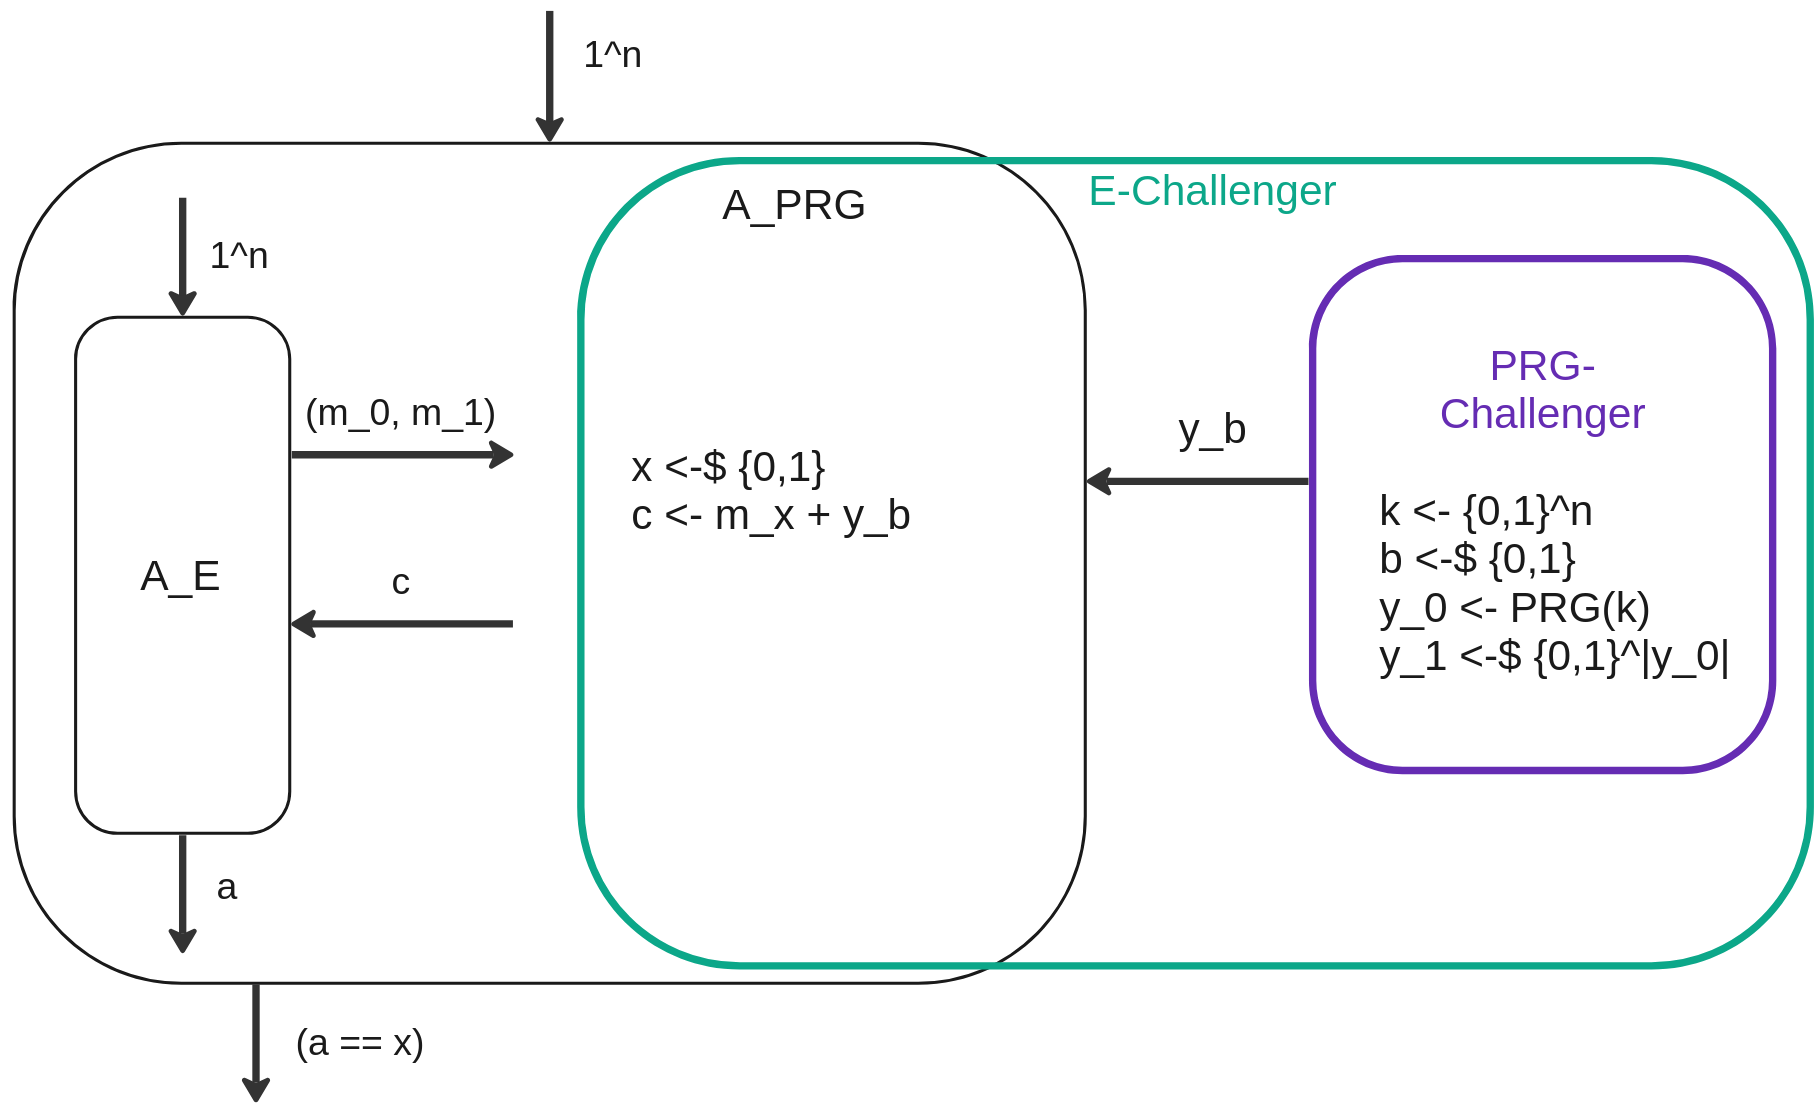
\includegraphics[width=\linewidth]{gfx/reduction_prg_key_expansion.png}
    \caption{Reduction for proving the IND-security of $\mathcal{E}$ if the IND-Security of PRG is given.}
    \label{fig:reduction_key_expansion}
\end{figure}


\section{Indistinguishability Under Chosen Plaintext Attack (IND-CPA)}

CPA is an attack model in which the attacker can retrieve ciphertexts for arbitrarily chosen plain texts as many times as he wants. But because the attacker must be efficient, he can just retrieve a polynomial amount of ciphertexts. The game-based definition of IND-CPA security is identical to the definition of IND security but allows requesting $c_b$ multiple times for different message pairs $(m_0, m_1)$. But the encryption oracle will have to choose $b$ once in the beginning and then keep it the same for each request.

Every IND-CPA-secure method is also IND-secure. But IND-secure methods are not automatically IND-CPA secure. For example, the OTP with the same key for each message is IND secure but not IND-CPA secure: An attacker could request the ciphertext for two message pairs $(m_0, m_1) \rightarrow c_1$ and $(m_0, m_2) \rightarrow c_2$. The attacker knows that if $b=0$, the oracle has encrypted $m_0$ two times and will therefore return $0$ if $c1 == c2$. If $b=2$, the oracle must have encrypted two different messages, which must because of correctness be mapped to different ciphertexts. Therefore, the attacker returns $1$ if $c_1 \neq c_2$.

An approach for making an encryption method using a secure PRG IND-CPA secure could be the following:\\
For each message to encrypt, call the PRG first to generate a key that is twice as long as the fixed-size message length. Then use the first half of the PRG output for encryption and save the second part. The first seed for the PRG will be taken from a $KGen$ algorithm. The following keys will be the second half of the PRG in the previous iteration. Because the PRG output is pseudo-randomized, it is also a secure seed.\\
This approach is nice, but it is not practicable, because the sender and the receiver must be synchronized, which might fail because of insecure connections with message retransmissions.

%%%%%%%%%%%%%%%%%%%%%%%%%%%%%%%%%%%%%%%
\section{Pseudo Random Functions (PRF) (Exercise 5)}
%%%%%%%%%%%%%%%%%%%%%%%%%%%%%%%%%%%%%%%

A PRF $PRF :=  K \times \{0,1\}^{in(\gamma)} \rightarrow \{0,1\}^{out(\gamma)}$ is a family of functions. When choosing a concrete $k$, the resulting function $f \in F$ is a pseudo-random function. For different key values, the function behaves like a different pseudo-random function.

Another way to explain this is that a PRF is a function $F(k,x) \rightarrow y$, which takes a (secret) key and a seed an $x$-value as input and produces a pseudo-random output with the following characteristics:

\begin{itemize}
    \item $y_0$ and $y_1$, generated as $F(k,x_0) \rightarrow y_0$ and $F(k,x_0) \rightarrow y_0$, are different, if $x_0 \neq x_1$ and are equal if $x_0 = x_1$.
    \item A CPA attacker cannot distinguish the output of a PRF from a truly random function, which would do the same thing but in a truly randomized fashion.
\end{itemize}

A PRF with equal input and output length is called length-preserving.

Defining a (secure) PRF using a game would involve creating a challenger which randomly chooses a hidden bit $b$ and, depending on that bit, calls the PRF or a truly random function. For both, the truly random function and the PRF, the outputs must be deterministic (consistent), such that if the same $x$ value is provided as input, the same $y$ value will be emitted.

%%%%%%%%%%%%%%%%%%%%%%%%%%%%%%%%%%%%%%%
\section{Pseudo Random Permutations (PRPs) (Exercise 6)}
%%%%%%%%%%%%%%%%%%%%%%%%%%%%%%%%%%%%%%%

A pseudo-random permutation is, similar to a pseudo-random function, a family of functions, which a concrete function can be selected from by choosing a key. A pseudo-random permutation is defined as $\{0,1\}^s \times \{0,1\}^l \rightarrow \{0,1\}^l$ with the key length $s$, and the input and output length $l$. The input space and the output space of a PRP are equal and the PRP defines a bijective permutation on the set of input bit strings (not on the set of input bits), making a PRP an invertible function. In other words, every possible bitstring is mapped to another bitstring of the same length. Each output bitstring belongs to exactly one input bitstring. Every PRP is a length-preserving PRF.

A \textit{secure} (weak \textit{PRP}) is defined just like the definition for the secure PRF (as it is also a PRF).

In contrast to PRFs and PRGs, PRPs also have a \textit{strong} security definition.
A PRP is strong if is secure under chosen plain text attacks if the attacker can access the PRP and its inverted operation PRP$^{-1}$.
The game-based CPA-IND definition states that, for a chosen bitstring, a distinguisher $D$ cannot distinguish the PRPs output of $f(x)$ or $f^{-1}(x)$ from the output of a real random permutation or its inverse operation.

%%%%%%%%%%%%%%%%%%%%%%%%%%%%%%%%%%%%%%%
\section{Data Encryption Standard (DES)}
%%%%%%%%%%%%%%%%%%%%%%%%%%%%%%%%%%%%%%%

DES is a block cipher, which was used until about the year 2000. Because of its short keys, it was later replaced with DES3 and eventually by AES.

\begin{wrapfigure}{r}{0.33\textwidth}
    \begin{center}
        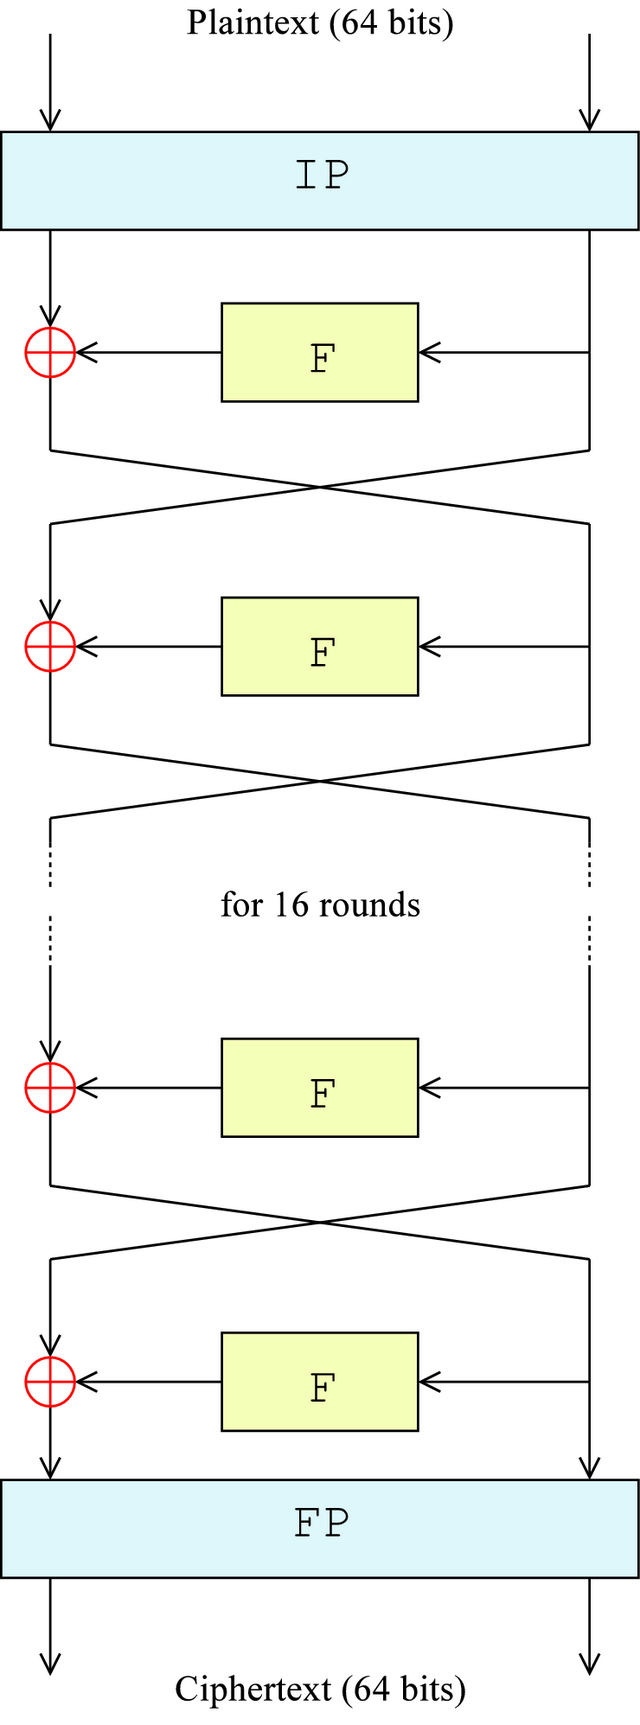
\includegraphics[width=0.33\textwidth]{gfx/feistel_function.png}
    \end{center}
    \caption{Feistel Function}
    \label{fig:feistel}
\end{wrapfigure}

DES defines an encryption method for encrypting 64-bit plain texts using 56-bit keys (the key is 64 bits long, but 8 bits are used for parity). It uses a so-called Feistel function in 16 rounds, where in each round a part of the key is used.

The Feistel function uses another function $F$ to operate on half of the 64-bit block at a time. Its most important characteristic is, that it is reversible, even if the internally used function $F$ is not reversible (e.g. a one-way hash function, which also has collisions).\\
In each iteration of the Feistel function, the plain text will be split in half ($L_i||R_i$) and transformed to a new intermediate ciphertext $L_{i+1}||R_{i+1}$ as follows:

\begin{align*}
    L_{i+1} & := R_i                   \\
    R_{i+1} & := F(k_i,R_i) \oplus L_i
\end{align*}

The exception is the last iteration, in which the sides will not be switched, such that $L{i+1} = F(k_i,R_i) + L_i$ and $R_{i+1} = R_i$.

Regardless of the function $F$, the Feistel function can be reversed by applying it again with reversed key order. That is possible because for each iteration we can compute $L_i$ from $R_{i+1} + L_{i+1}$ and can take $R_i$ directly from $L_{i+1}$.

The Feistel function provides the reversibility of the function, however, it does not provide the security itself. The security is provided by the internally utilized function $F$. In DES this function is using so-called S- and P-boxes, whose details go beyond the scope of this course. What is important, however, is that $F$ implements Shannon's Concept of \textit{confusion and diffusion} and that it takes a part of the key $k_i$ and a bitstring as an input. The function $F$ is, in fact, a non-reversible function.

56 bits ($2^{56}$ possibilities) were soon not sufficient for security against brute-force attackers on modern hardware. What could have been done to increase its security would be creating a new encryption algorithm, which works like DES but uses a longer key. But to reduce the effort required to increase DES's security, another approach was used \textendash{} applying DES multiple times with different keys.

The first approach would be to compute DES two times with two different keys to achieve the security of $2^{112}$, because brute force a ciphertext, the attacker would have to compute all possible combinations of keys of the first DES and keys of the second DES $2^{56} \cdot 2^{56}$. But if an attacker would know the plain text $m$ and the ciphertext $c$ of a message, he could use a \textit{meet-in-the-middle} attack to drastically reduce the computational effort for brute forcing. In the following, the computation of double DES is shown:

$$
    m \rightarrow DES_{1}(key_1, m) \rightarrow c' \rightarrow DES_{2}(key_2, c') \rightarrow c
$$

An attacker could then first compute all possible intermediate ciphertexts $c'$ for all possible values of $k_1$ from $m$ and save the results in a hashmap. Then he could compute all possible intermediate ciphertexts $c'$ with all possible values of $k_2$ from $c$ using $DES_2^{-1}$. The computation required is equal to $2^{56} + 2^{56} = 2 \cdot 2^{56} = 2^{57}$ instead of $2^{112}$. To obtain the correct combination of $k_1$ and $k_2$, the attacker would then search for collisions i.e. for pairs $(k_1, k_2)$ that produced the same intermediate ciphertext $c'$.

For this reason, double DES is not useful. Instead, Triple DES is used, which has the security of $2^{112}$, because the attacker can use a meet-in-the-middle attack but has to calculate two DES on one of the sides. Triple DES uses the inverse operation (reverse order key parts of $k_2$) of $DES_2$ for the second DES. The reason is that there was uncertainty about whether DES could be a \textit{group}, such that there might be one $DES_{x}$ operation, which would be equal to the combination of $DES$ one to three. Later, however, it was discovered, that DES is not a group and inverting the middle DES was, therefore, not required:

$$
    m \rightarrow DES_{1}(key_1, m) \rightarrow c' \rightarrow DES^{-1}_{2}(key_2, c') \rightarrow c'' \rightarrow DES_{3}(key_3, c'') \rightarrow c
$$

%%%%%%%%%%%%%%%%%%%%%%%%%%%%%%%%%%%%%%%%%%%
\section{Advanced Encryption Standard (AES) (Exercise 6)}
%%%%%%%%%%%%%%%%%%%%%%%%%%%%%%%%%%%%%%%%%%%

The security of DES (56-bit keys) and DES3 (112-bit security) is not sufficient. For this reason, the NIST started a public challenge for creating a cryptographic process replacing DES in 1979. The winner of this contest was decided to be Rijndael in 2000, which is the basis for the nowadays used advanced encryption standard (AES). AES is Rijndael, which can generally work with different input and output sizes (block sizes), with a block size of 128-bit. The key length for AES can be chosen to be 128, 192 or 256-bit.

AES is a substitution permutation network. This means it tries to replace bits with other bits (substitution) and change the order of bits (permutation)\footnote{Note that here permutation is a permutation on the set of bits, whereas the \textit{permutation} in PRP refers to a permutation on the set of the different bit strings.}.

AES takes a 128-bit string as input and stores it as a $4 \times 4$ two-dimensional matrix, where each element is an 8-bit substring. Then it executes the following operations on the matrix for a minimum of 10 rounds\footnote{The number of rounds can be greater if longer keys are used.}:

\begin{itemize}
    \item \textit{AddRoundKey:} The round key, which is a substring of the expanded input key, is added ($\oplus$) to the message.
    \item \textit{SubBytes:} Every byte is replaced by another byte according to a fixed replacement scheme (S-box).
    \item \textit{ShiftRows:} The bytes of each row are shifted depending on the row number (row 0 is not shifted, row 1 is shifted 1 element, ...).
    \item \textit{MixColumns:} Same as ShiftRows but for columns.
\end{itemize}

In the last round, AddRoundKey is executed instead of MixColumns. SubBytes is the substitution and ShiftRows and MixColumns are the permutation of the substitution permutation network.

AES is an IND-CPA secure PRP (and therefore also an IND-CPA secure PRF).

%%%%%%%%%%%%%%%%%%%%%%%%%%%%%%%%%%%%%%%%%%%
\section{Block Cipher Modes of Operation (Exercise 6)}
%%%%%%%%%%%%%%%%%%%%%%%%%%%%%%%%%%%%%%%%%%%

The main characteristic of block ciphers is that they can only encrypt bit strings of fixed size.
However, the message size is usually variable and greater than the input size of the block cipher.
Therefore, a method is needed to use block ciphers for messages with arbitrary lengths.
Generally speaking, messages are divided into chunks that match the input length of the block cipher used.
Then the mode of operation provides a schema for the encryption of the individual blocks utilizing a block cipher.
If the message length is not a multiple of the block cipher's input length, padding must be added to the last block of the plain text message before encrypting. Usually, this will be a $1$ followed by the required number of zeroes. This way, the padding can be identified after decrypting by removing all zeroes from the right side until a $1$ appears.

% TODO: add pictures here 

%%%%%%%%%%%%%%%%%%%%%%%%%%%%%%%%%%%%%%%%
\subsection{Electronic Code Book (ECB)}
%%%%%%%%%%%%%%%%%%%%%%%%%%%%%%%%%%%%%%%%

This is the simplest mode of operation. It encrypts every part of the message independently with the same unmodified key. This is not IND-CPA secure, because equal plain text blocks are encrypted to equal ciphertext blocks.\footnote{For formal proof of insecurity, see the solution of exercise sheet 6.}

\begin{figure}
    \center
    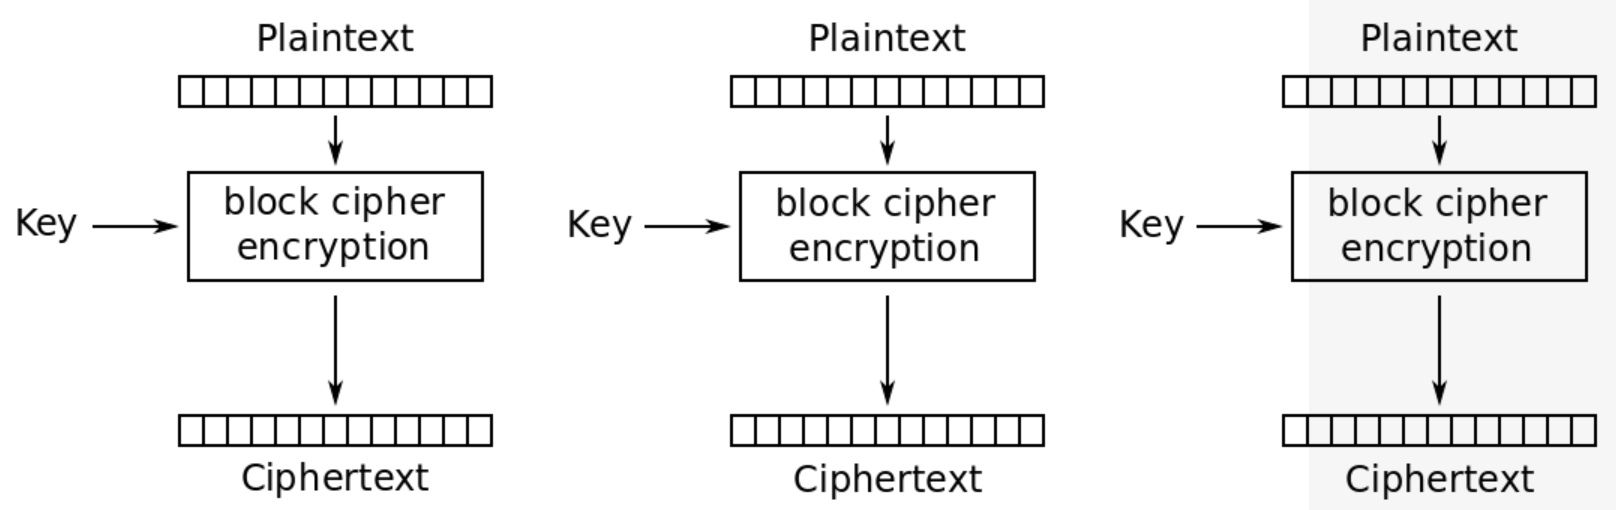
\includegraphics[width=\linewidth]{gfx/ecb_enc_scheme.png}
    \caption{ECB Encryption}
    \label{fig:ecb_enc}
\end{figure}

\begin{figure}
    \center
    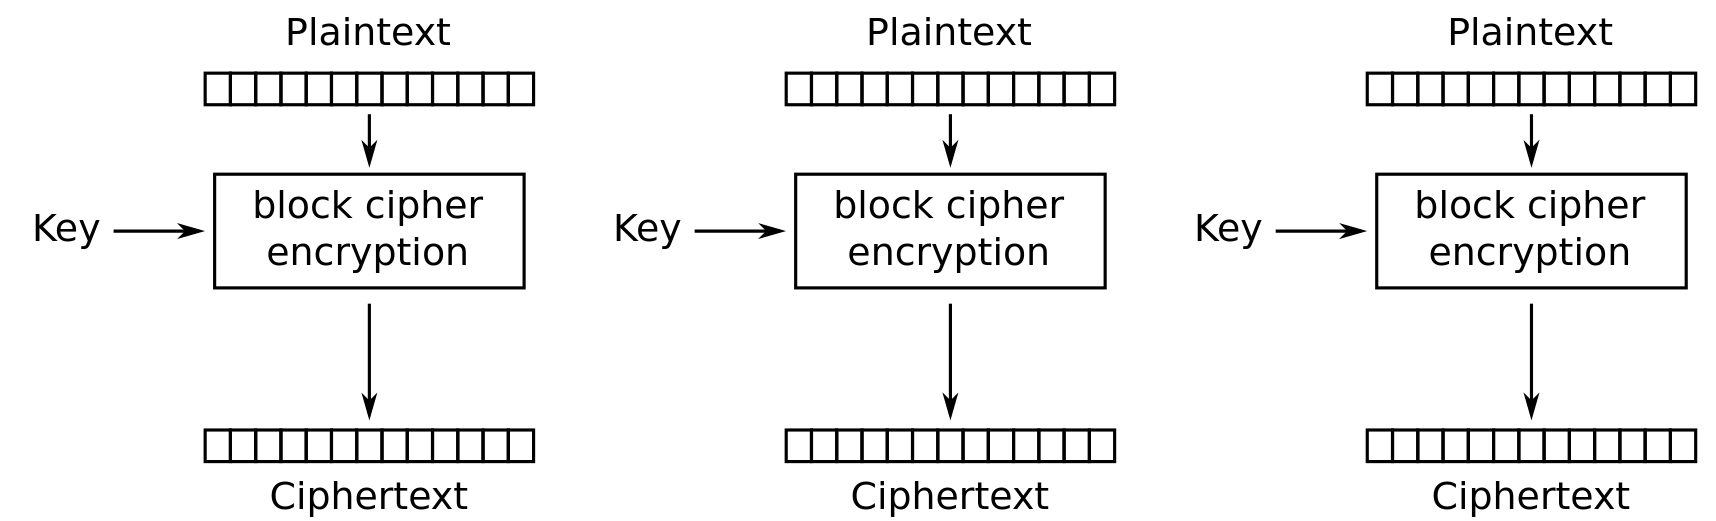
\includegraphics[width=\linewidth]{gfx/ECB_dec_scheme.png}
    \caption{ECB Decryption}
    \label{fig:ecb_dec}
\end{figure}

%%%%%%%%%%%%%%%%%%%%%%%%%%%%%%%%%%%%%%%%
\subsection{Cipher Block Chaining (CBC)}
%%%%%%%%%%%%%%%%%%%%%%%%%%%%%%%%%%%%%%%%

Cipher block chaining adds ($\oplus$) the previous cipher block to the message before applying the block cipher in each step. Because the cipher blocks are pseudo-random, the input to the block cipher is also pseudo-random, which makes it output pseudo-random. Because for the first block, there is no previous cipher text block, a random initialization vector $IV$ is used. CBC is IND-CPA secure.

\begin{figure}[h]
    \center
    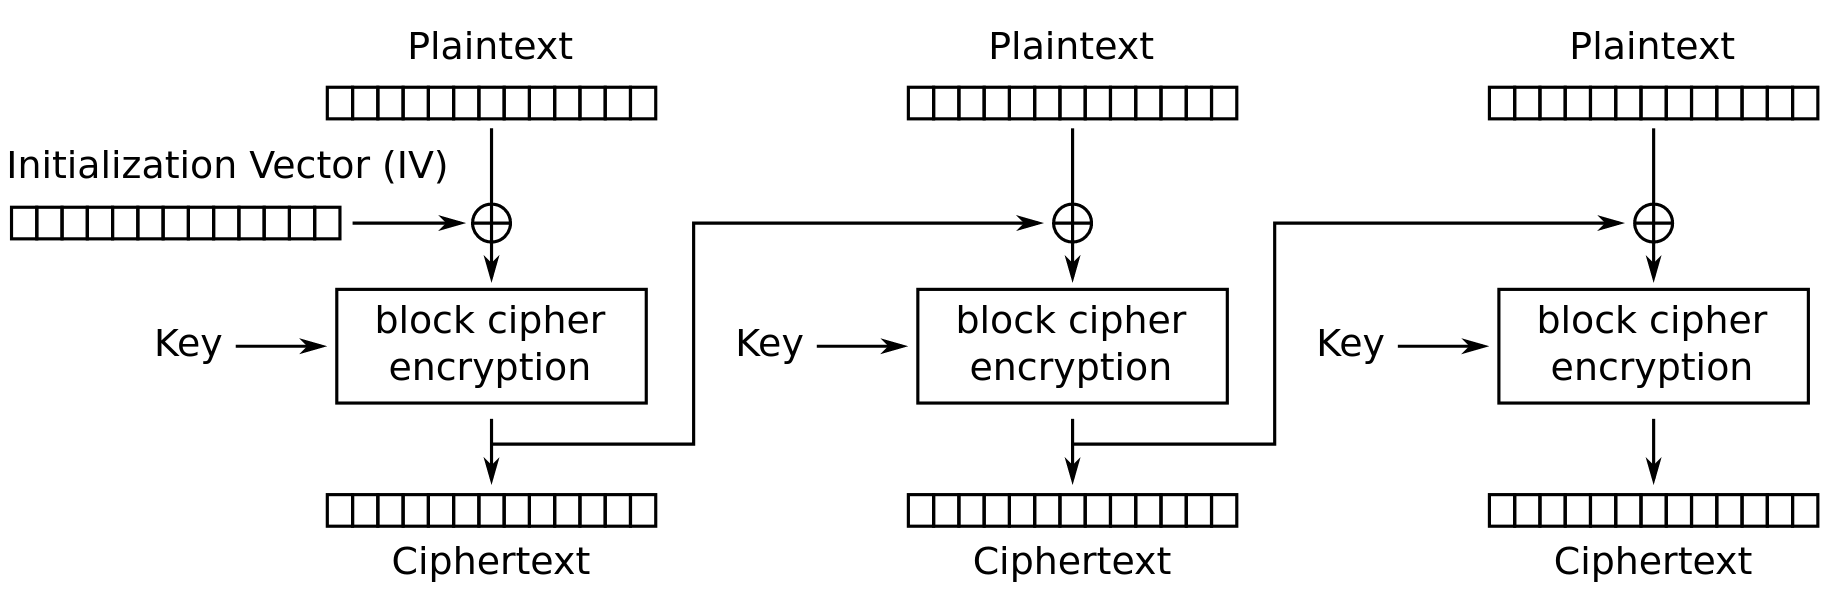
\includegraphics[width=\linewidth]{gfx/CBC_enc_scheme.png}
    \caption{CBC Encryption}
    \label{fig:cbc_enc}
\end{figure}

\begin{figure}[h]
    \center
    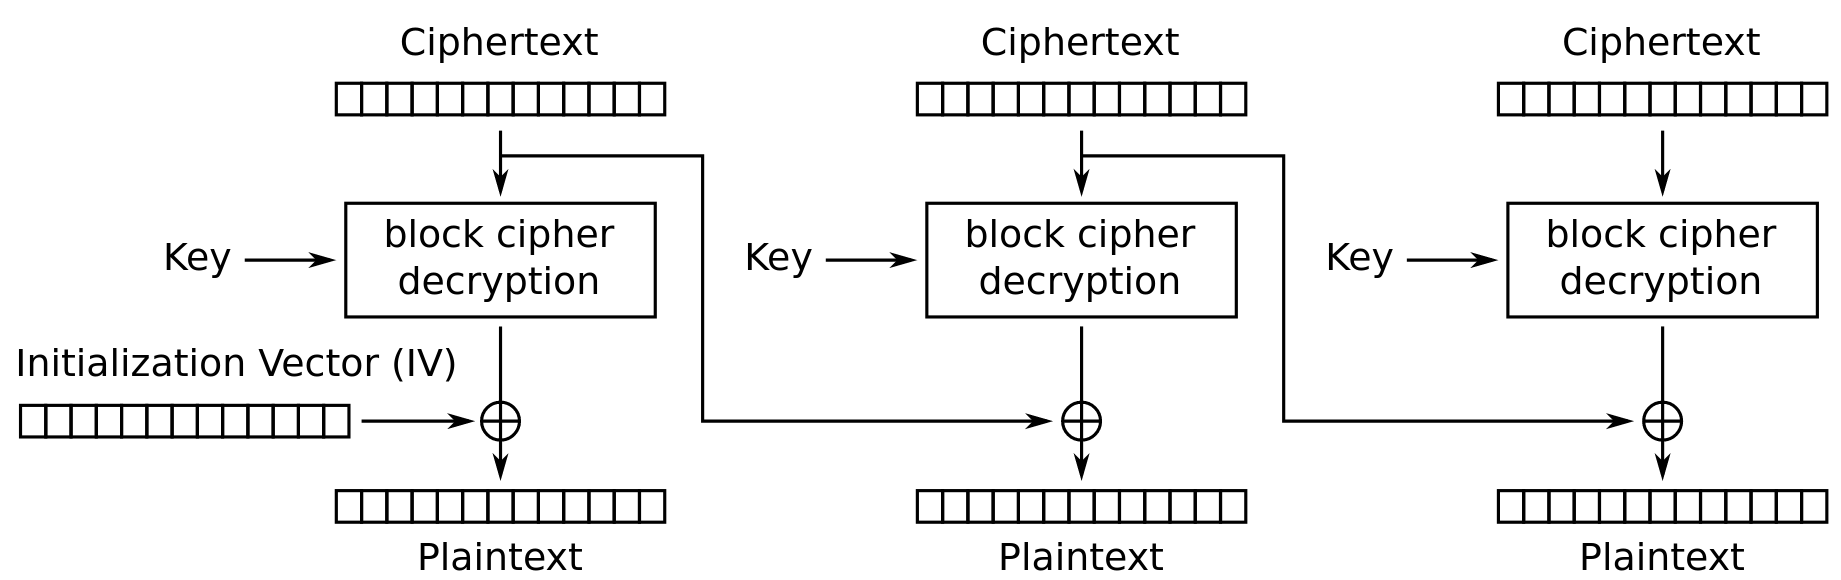
\includegraphics[width=\linewidth]{gfx/CBC_dec_scheme.png}
    \caption{CBC Decryption}
    \label{fig:cbc_dec}
\end{figure}

\textbf{Advantages:}

\begin{itemize}
    \item Parallel Decryption is possible
    \item Loss of a cipher block $c_i$ during transmission only affects plain text blocks $m$ and $m+1$ after decryption (minor advantage)
\end{itemize}

\textbf{Disadvantages:}

\begin{itemize}
    \item Encryption can only happen sequentially
    \item Decryption requires inverse block cipher
\end{itemize}

%%%%%%%%%%%%%%%%%%%%%%%%%%%%%%%%%%%%%%%%
\subsection{Output Feedback Mode (OFB)}
%%%%%%%%%%%%%%%%%%%%%%%%%%%%%%%%%%%%%%%%

The OFB uses the output of the block cipher of the previous iteration as input to the block cipher of each iteration. Because the previous output of the block cipher is pseudo-random, the output of each block cipher is pseudo-random. OFB is IND-CPA secure.

\begin{figure}[h]
    \center
    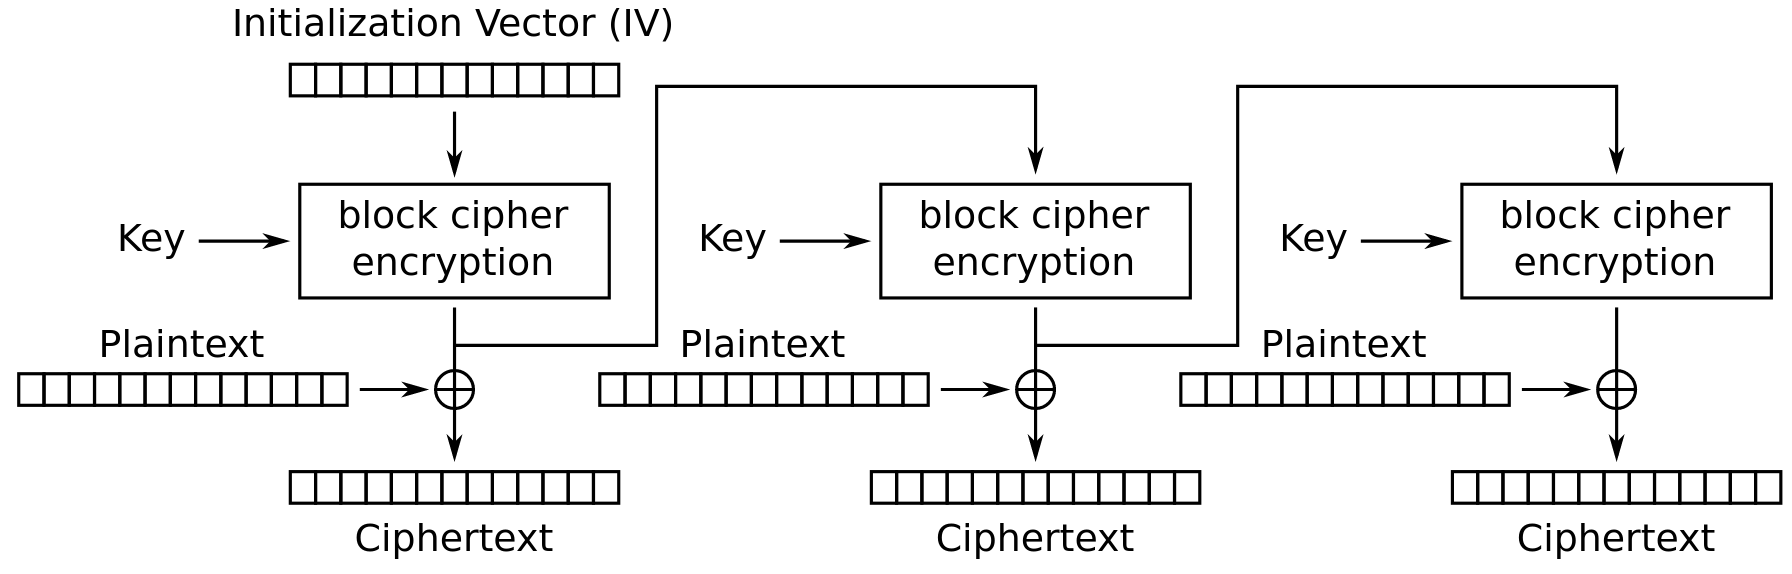
\includegraphics[width=\linewidth]{gfx/OFB_enc_scheme.png}
    \caption{OFB Encryption}
    \label{fig:ofb_enc}
\end{figure}

\begin{figure}[h]
    \center
    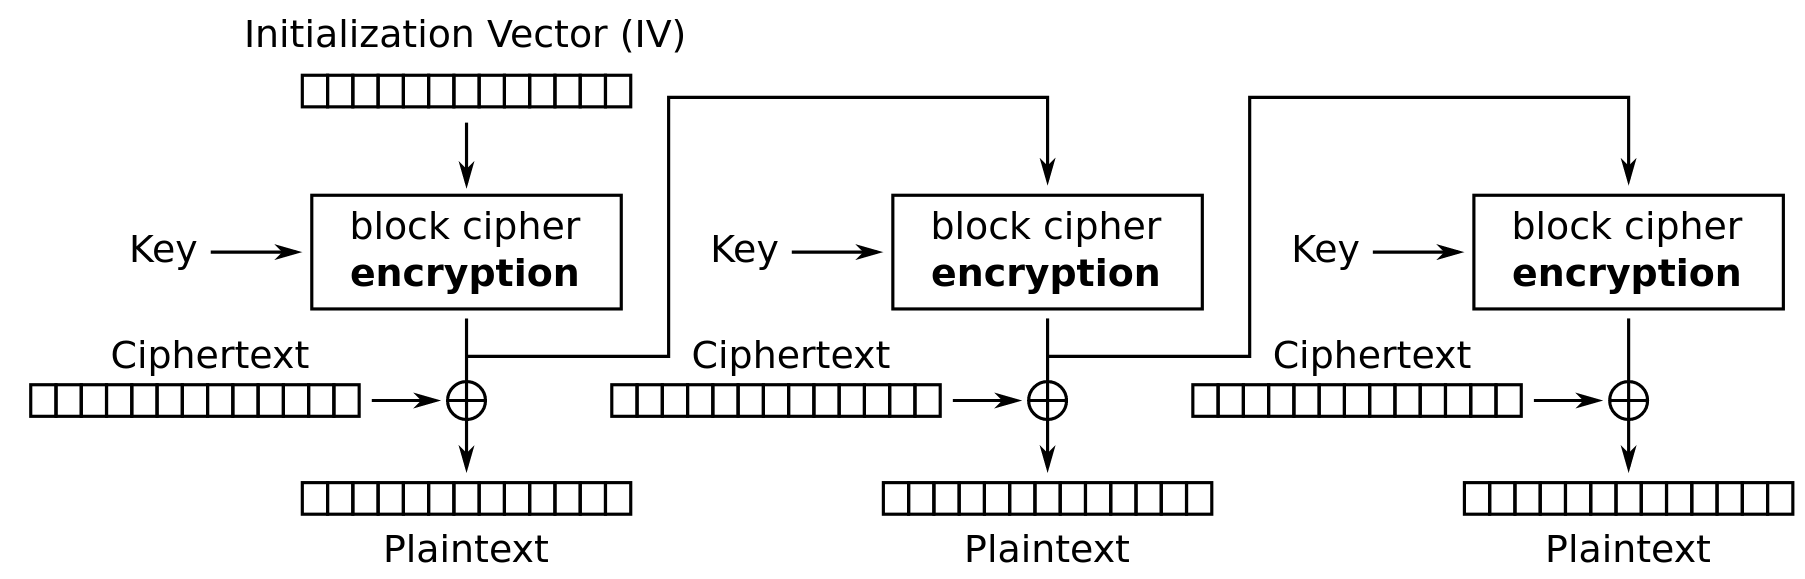
\includegraphics[width=\linewidth]{gfx/OFB_dec_scheme.png}
    \caption{OFB Decryption}
    \label{fig:ofb_dec}
\end{figure}

\textbf{Advantages:}

\begin{itemize}
    \item No inverse operation of the block cipher is required
    \item No padding is required
    \item The block cipher output can be precalculated because it does not depend on the message. As soon as a message arrives, the block-cipher output can be added ($\oplus$) to the message (in parallel possible).
\end{itemize}

\textbf{Disadvantages:}

\begin{itemize}
    \item Encryption and Decryption can only happen sequentially
\end{itemize}

%%%%%%%%%%%%%%%%%%%%%%%%%%%%%%%%%%%%%%%%
\subsection{Cipher Feedback (CFB)}
%%%%%%%%%%%%%%%%%%%%%%%%%%%%%%%%%%%%%%%%

CFB is a variant of OFB.
Instead of using the output of the block cipher as the input of the next block cipher, the ciphertext block is taken as the next input to the block cipher.
The advantages and disadvantages are the same as those of OFB.

\begin{figure}[h]
    \center
    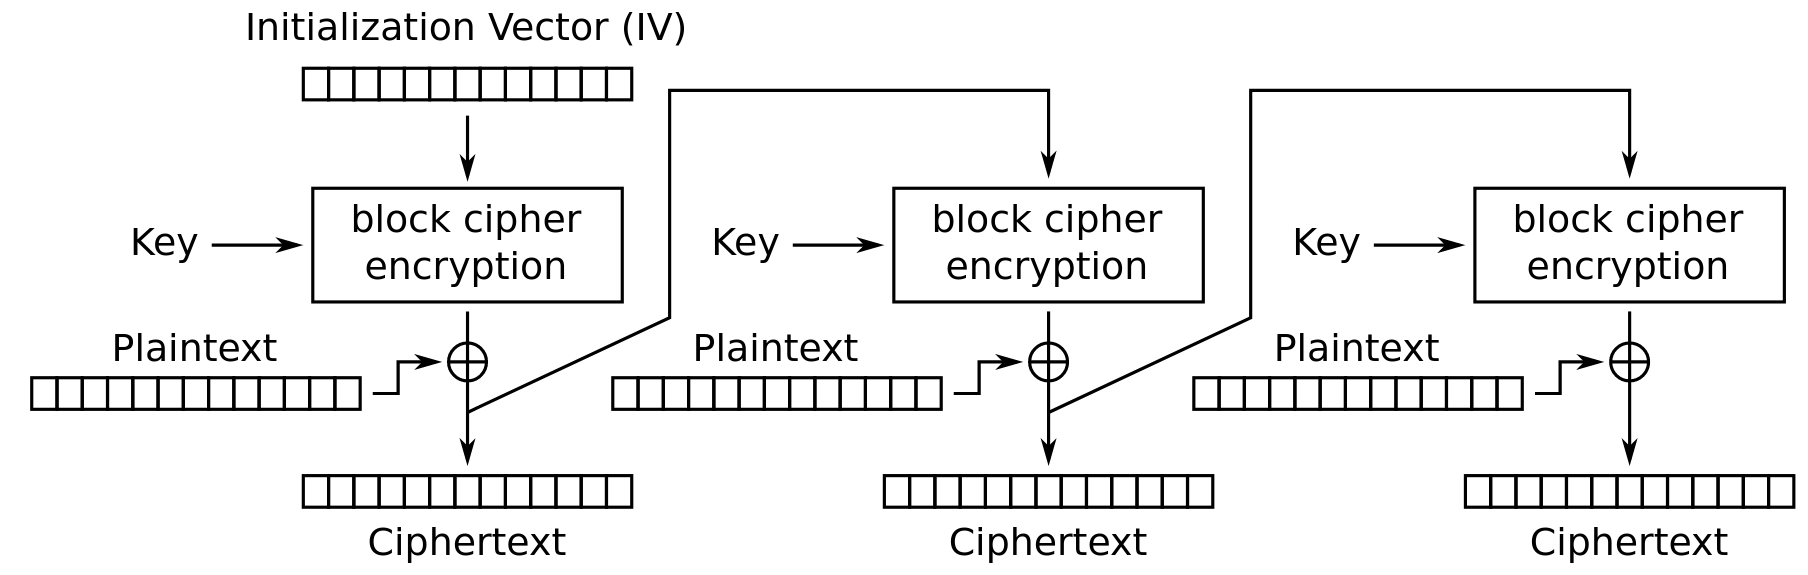
\includegraphics[width=\linewidth]{gfx/cfb_enc.png}
    \caption{CFB Encryption}
    \label{fig:cfb_enc}
\end{figure}

\begin{figure}[h]
    \center
    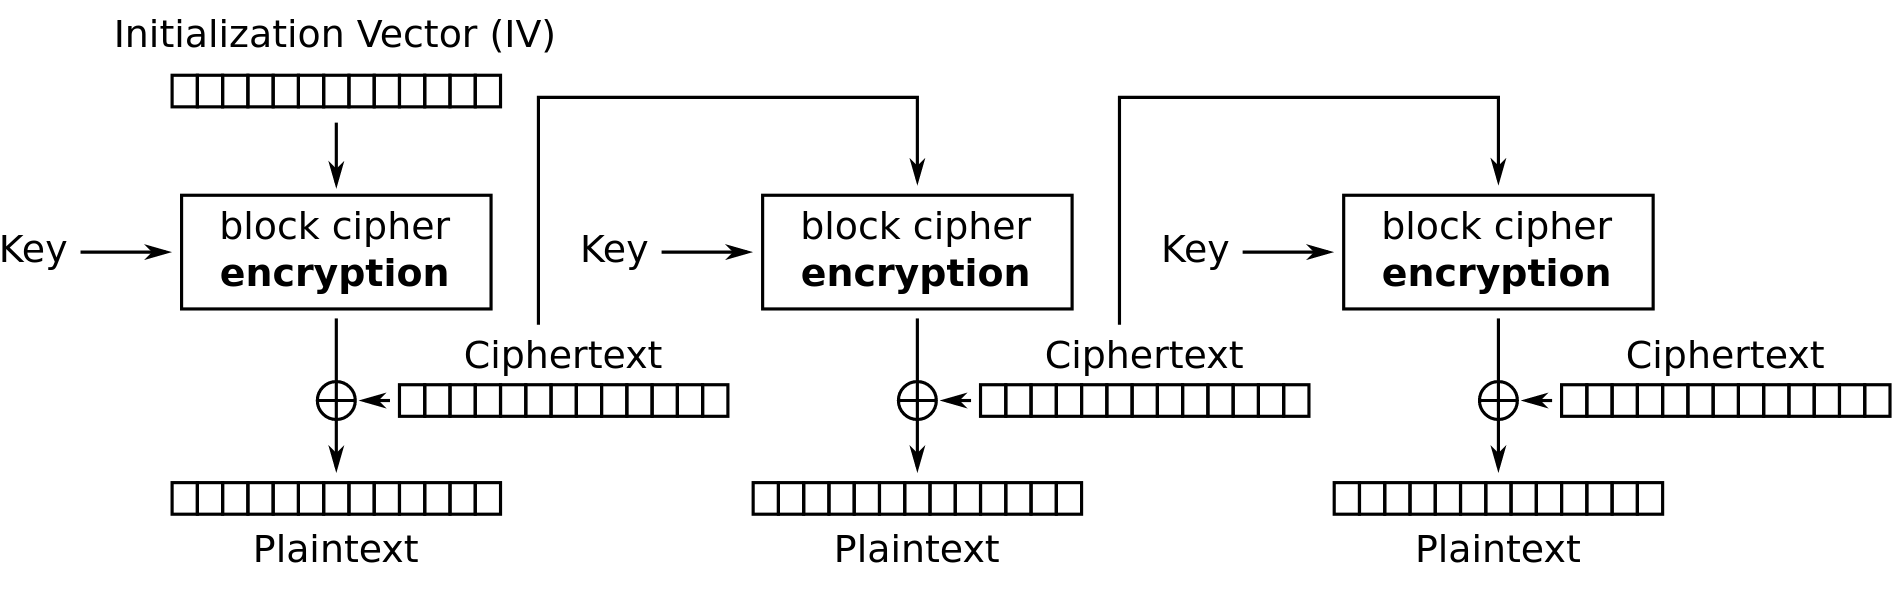
\includegraphics[width=\linewidth]{gfx/cfb_dec.png}
    \caption{CFB Decryption}
    \label{fig:cfb_dec}
\end{figure}

%%%%%%%%%%%%%%%%%%%%%%%%%%%%%%%%%%%%%%%%
\subsection{Counter Mode (CTR)}
%%%%%%%%%%%%%%%%%%%%%%%%%%%%%%%%%%%%%%%%

The counter mode uses a combination of a key (here called initialization vector or Nonce) and a counter.

\begin{figure}[h]
    \center
    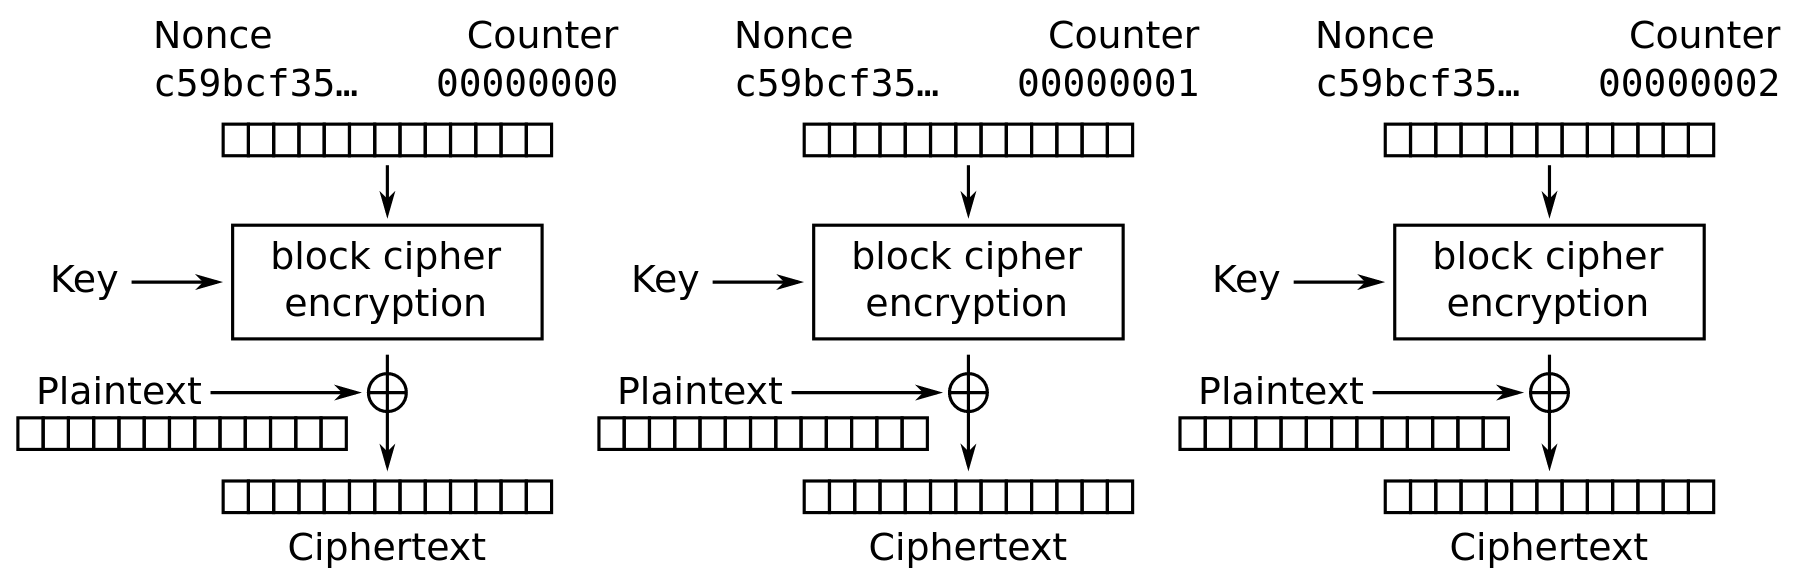
\includegraphics[width=\linewidth]{gfx/enc_ctr.png}
    \caption{CTR Encryption (Decryption analogous, switch plain text and cipher text)}
    \label{fig:ctr_enc}
\end{figure}

\textbf{Advantages:}

\begin{itemize}
    \item Fully parallelizable encryption and decryption
    \item Transmission error in cipher text block $c_i$ only affects plain text block $m_i$
    \item No padding for last plain text block necessary
    \item No inverse operation of the block cipher is required
\end{itemize}

\textbf{Disadvantages:}

\begin{itemize}
    \item Security is reduced by the number of bits that are used as counter bits.
\end{itemize}

%%%%%%%%%%%%%%%%%%%%%%%%%%%%%%%%%%%%%%%%%%%%%%%%
\section{Message Authentication Codes and EUF-CMA}
%%%%%%%%%%%%%%%%%%%%%%%%%%%%%%%%%%%%%%%%%%%%%%%%

Encryption methods only ensure \emph{confidentiality} and are not enough to ensure secure communication. What we want to do is to complement confidentiality with \emph{integrity} and \emph{authenticity}. These properties can be achieved by using \acp{MAC}. \acp{MAC} are checksums that include a secret key in their calculation. That way, if the \ac{MAC} is secure, the receiver of a message can be sure that the message has not been modified if the provided checksum is valid since no attacker can create a matching checksum for a modified message without knowing the secret key.

The security of a \ac{MAC} is defined through the game-based definition of EUF-CMA, which stands for existential unforgeability under chosen message attacks. The attacker $A$ can query as many \acp{MAC} from the \ac{MAC} oracle as it wants. Eventually, $A$ must emit a pair $(m,\tau)$ of a message and a corresponding \ac{MAC}. The attacker $A$ is successful if $\tau$ matches the message $m$ and if the message $m$ has not been queried before.

A slightly stronger variant of EUF-CMA is sEUF-CMA (\emph{strong} EUF-CMA). A \ac{MAC} is sEUF-CMA if the attacker $A$ also wins the game if it finds another \ac{MAC} that is valid for a queried message $m$. That means that the requirements for the attacker's output are less strict. It is not required that the message $m$ has not been queried before, but only that the pair $(m,\tau)$ has not been queried before. Since this gives the attacker additional opportunities to break the \ac{MAC}, the \ac{MAC} must be more secure.

%-------------------------------------------------
\section{PRF-MAC}
%-------------------------------------------------

Every pseudo-random function is also a MAC for messages \emph{with the size of its input length}.
To realize that, the MAC for a message $m$ is calculated by using the PRFs function value at position $m$ using the key $k$ as $MAC := PRF(k,m)$.
To break this MAC an attacker would have to guess the value of a strong PRF without knowing the key, which is not possible.
Hence, the security of PRF-MACs can be proved using a reduction to the IND-CPA security of the used PRF.

%-------------------------------------------------
\section{CBC-MAC}
%-------------------------------------------------

To overcome the limitations that PRF-MAC has for the input message's length, MACs built based on block ciphers can be used.
The block cipher is calculated for the entire message.
Then the last ciphertext block is emitted.
We had seen earlier that the security of block ciphers requires a \emph{random} initialization vector $IV$.
This is different when building MACs based on block ciphers.
Since the first ciphertext block is not transmitted, the receiver would not have a chance to recalculate the MAC as the information about the $IV$ is not transmitted.
One could decide to transmit the $IV$ as well. This, however, would allow the attacker to modify the message and the $IV$, which may allow him to find a matching MAC for the modified message when using the modified $IV$.
Hence, CBC-MACs using random $IV$s and transmitting them are not secure.
Instead, CBC-MACs should use a \emph{constant} $IV$ (usually just $0^\lambda$, which is equivalent to no $IV$).

% TODO: insecurity of CBC mac with different message sizes (01:10:40)

% TODO: CBC-MAC implementation from US government


%-------------------------------------------------
\section{HMAC}
%-------------------------------------------------
\chapter{Public-Key Cryptography}\label{ch:pub_key_crypto}

%------------------------------------------
\section{Introduction}\label{sec:pubkey:intro}
%------------------------------------------

Public-key methods use the following functions for encrypting and decrypting:

\begin{align*}
    KGen(1^n)  & \rightarrow (sk, pk) \\
    Enc(pk, m) & \rightarrow c        \\
    Dec(sk, c) & \rightarrow m        \\
\end{align*}

Often, the public key can be computed efficiently from the secret key $f(pk) \rightarrow sk$.
But for security, it is required that the reverse of this function $f^{-1}$, which computes the secret key from the public key is \emph{not} efficiently computable.
We call such a function, that can only be efficiently computed in one direction a \emph{one-way function} (OWF).

%----------------------------------------
\section{One-Way Functions}\label{sec:owf}
%----------------------------------------

A one-way function (OWF) is a function $f: \{0,1\}^* \rightarrow \{0,1\}*$ that can be efficiently computed but its inverse function cannot be efficiently computed.

Formally speaking, a function $f$ is one-way if it has the following two properties:

\begin{enumerate}
    \item There is an efficient algorithm PPT for computing values $f(x)$ for all allowed input parameters $x$.
    \item For all efficient PPT algorithms A their success probability in the below security game $G^{inv}_{f,A}$ is negligible.
\end{enumerate}

$G^{inv}_{f,A}$ is defined as follows:

\begin{align*}
    \{0,1\}^\lambda & \$\rightarrow x \\
    f (x)           & \rightarrow y   \\
    A(1^\lambda, y) & \rightarrow x'  \\
    return f(x) == x'
\end{align*}

\textbf{Note 1:} This game does not require the adversary $A$ to find the value $x$ used but merely requires it to find a value that produces the output for $f$ i.e. a collision.

\textbf{Note 2:} This assumes that there are problems that are hard to compute (NP-hard). This is an assumption that holds so far but is not proven.

%---------------------------------------------
\section{Number Theory}\label{sec:number_theory}
%---------------------------------------------

\subsection{The Modulo Operator}

The modulo operator allows us to calculate with residual rings, which means that all values will never exceed the number $m-1$ for a residual ring $Z_m$.
We define addition and multiplication, such that they produce a value $x \in Z_m$ such that:

\begin{align*}
    a + b & = c mod m \quad |\quad \exists i \in Z: \quad a + b = c + i \cdot m     \\
    a + b & = c mod m \quad |\quad \exists i \in Z: \quad a \cdot b = c + i \cdot m
\end{align*}

\subsection{Groups}

A group is a combination $(G,\circ)$ of a set $G$ and an operation $\circ$ with the following 4 characteristics:

\begin{itemize}
    \item Closure: $a \circ b \in G \quad | \quad \forall a,b \in G$
    \item Associativity: $a \circ (b \circ c) = (a \circ b) \circ c \quad \forall a,b,c \in G$
    \item There exists an identity element (neutral element) $n$ such that $a \circ n = n \circ a = a \quad \forall a \in G$
    \item There exists an inverse element $a^{-1}$ for all elements $a$ in $G$ that can turn $a$ into the neutral element if combined with the operation $\circ$: $\exists a^{-1} \in G: \quad a \circ a^{-1} = a^{-1} \circ a = n \quad \forall a \in G$.
\end{itemize}

We call a group an abelian group if it is a group for which the operation $\circ$ over $G$ is commutative for all elements in $G$:
$a \circ b = b \circ a \quad \forall a,b \in G$.

Groups, or abelian groups, are nice to work with in cryptography.
Unfortunately, residual rings $Z_m$ are generally not groups if paired with the multiplication operator $(Z_m,\cdot)$ because they do not have inverse elements for all elements in $Z_m$. For example, each group $Z_m$ contains the value $0$, but no number can be multiplied by $0$ to produce the neutral element, which is $1$.
Additionally, depending on $m$, other elements might have no inverse element as well.

For this reason, we would like to reduce the set $Z$ to a set $Z_m^*$ that only contains all invertible elements of $Z_m$, thus making it a group.
The invertible elements of $Z_m$ are exactly all elements for which the greatest common divisor ($gcd$) is equal to $0$.
For instance, for the residual ring $Z_6 = \{0, 1, 2, 3, 4, 5\}$, the reduced group would be $Z_6^* = \{1, 5 \}$.

The number of elements in $Z_m^*$ is well defined for a couple of cases for prime numbers $p,q$ and positive integers $k$:

\begin{itemize}
    \item $|Z_p^*| = p-1$ (all elements of $Z_m$ except $0$)
    \item $|Z_{p^k}^*| = p^k - \frac{p^k}{p}$ (all elements except all multiples of p in $Z_{p^k}$)
    \item $|Z_{p \cdot q}^*| = |Z_{p}^*| \cdot |Z_{q}^*|$\footnote{This can be proven as follows: $\Phi(p \cdot q) = p \cdot q - (p-1) - (q-1) - 1 = p \cdot q - (p-1) - q  + 1 - 1 = (p-1)q - (p-1) = (p-1) \cdot (q-1) = \Phi(p) \cdot \Phi(q)$. These are all elements contained in $Z_{p,q}$ except all multiples of $p$ (there are $q-1$ of those and $q$ (there are $p-1$ of those). And also the element $0$ has to be subtracted.}
\end{itemize}

\textit{Def:} The \emph{order} of a group $(G, \circ)$ is the number of the elements in $G$: $ord(G) = |G|$.

\textit{Def:} The \emph{order} of an element $a \in G$ of a group $(G, \circ)$ is the number of elements that can be generated by applying the operation $\circ$ to $a$ and $a$ in $G$.

\textit{Def:} A group $(G, \circ)$ is \emph{cyclic} there exists an element $g \in G$, which we call the generator of the group, that can generate all elements of the group. This means that $ord(g) = ord(G)$.
It can be proven all groups $(Z_p^*, \cdot)$ with prime numbers $p$ are cyclic.

In cryptography, we would like to have a group $(G, \cdot)$ that is cyclic \emph{and} has a prime number of elements.
If we choose $Z_p^*$ with a prime $p$, we have a cyclic group. But the group has $(p-1)$ elements, which itself is not a prime\footnote{Since all prime numbers $>3$ are uneven numbers, $p-1$ for $p>2$ is even, therefore divisible by two and, hence, not prime.}.
To find a group that is cyclic and has a prime order, we first find a group $(Z_p^*)$ for a prime $p = wq + 1$\footnote{Example: $11 = 2 \cdot 5 + 1$, $w$ can be any positive integer.}, where $p$ and $q$ are both primes.
Since $p$ is prime, there is a generator $a$ for $Z_p^*$.
We can now find a subgroup with the desired characteristics by finding a generator $g$ that generates a subgroup $<g>$ of $Z_m^*$ that has a prime number of elements.
We do that by defining the generator as $g := a^w mod p$.
$g$ is a generator that generates all $w$-th elements of the initial group because if it is multiplied with itself it skips multiples of $a$, e.g. $g^3$ is equivalent to $(a^w)^3 = a^3w$ and $a^1,a^2$ are skipped.
This means that a group $<g>$ generated by $g$ has one $w$-th of the elements that the initial group $Z_m^*$ had:
It follow that: $|<g>| = \frac{|Z_m^*|}{w} = \frac{wq + 1 - 1}{w} = q$.
Thus, the order of $<g>$ is also prime (because we defined $q$ as a prime earlier).

%----------------------------------------------
\subsection{Fermat's Little Theorem}\label{sec:little_fermat}
%----------------------------------------------

Fermat's little theorem states that for any positive integer $a$ and for any prime number $p$ the following holds:

$$
    a^p \equiv a \; mod \; p
$$

If the greatest common divisor of $a$ and $p$ is 1\footnote{Which is true for at least all $a < p$ because $p$ is prime}, it also follows that:

$$
    a^{p-1} = 1 \; mod \; p
$$

because if we multiplied both sides by $a$, we would end up at the original equation.

%----------------------------------------------------
\section{Discrete Logarithm Problem}\label{sec:discrete_log}
%----------------------------------------------------

Let $(G, \cdot)$ be a subgroup of $Z_p^*$ with prime order $q$, $g$ be a generator for the group and further $y \in G$ an element in the group.
The logarithm problem describes the task to find the (smallest) exponent for which $g$ generates $y$:

$$
    g^x \equiv y \; \text{in} \; G
$$

While solving this in the set of real numbers $R$ is easy, it is not easy for some groups with prime order.

The discrete logarithm assumption, which means that the discrete logarithm is hard to compute, is given for a group generator algorithm $Gen(1^\lambda)$ if all PPT algorithms win the below-defined game $Exp^{DL}_{Gen,A}$ only with negligible probability: $Pr[Exp^{DL}_{Gen,A}(1^\lambda) = 1] = neg(\lambda)$.

The game $Exp^{DL}_{Gen,A}(1^\lambda)$ is defined as follows:

\begin{align*}
    (G, q, g) & \leftarrow Gen(1^\lambda)           \\
    x         & \leftarrow^\$ \; G                  \\
    y         & \leftarrow g^x \; \text{in} \; G    \\
    x'        & \leftarrow A(1^\lambda, G, q, g, y) \\
    \text{return} \; [g^x \equiv y \; \text{in} \; G ]
\end{align*}

\section{Attacks Against The Discrete Logarithm}

In this section, we show the known attacks against the discrete logarithm on groups $G, q, p$, where $q$ is the order of the (sub)group and $p$ is the order of the (super)group, in which we are calculating the modulo.

\subsection{Brute Force}

Try all values $g^0, g^1, g^2, g^3 (...)$ until the value $g^i = y$ is found.

This trivial attack is on average not successful in an acceptable time because the adversary needs to try $\frac{1}{2} \cdot 2^\lambda$ of the possible $2^\lambda$ values on average. Therefore the runtime complexity is $O(\lambda)$

\subsection{Giant-step-baby-step algorithm}\label{sec:giant_baby}

\begin{enumerate}
    \item \textit{Giant-steps:} set $t = \sqrt{ord(G)}$. Then compute $t$ giant step values from $k=0$ to $k=(t-1)$ that can be generated from $G$ with the distance of $t$ to each other as:\\
          $g^{0t}, g^{1t}, g^{2t}, ... g^{t-1}$.
    \item The value $y$, of which we would like to find the discrete log to the base of $g$ is $g^x$ in $G$ and is located between two of the precomputed giant steps. Also, its distance to the next giant step will be less than $t$, because the giant steps all have the distance $t$. So we now compute all values that can be generated from $g$ starting at $y$ until we reach the next giant step:\\
          $y \cdot g^0, y \cdot g^1, y \cdot g^2 (...) \text{ until $y \cdot g^i$ matches one of the giant steps}$
    \item Since we then know the next giant step and in how many steps it can be generated from $g$, we know that $y$ can be generated in $i$ fewer steps from $g$:\\
          $x = k \cdot t - i$
\end{enumerate}

This algorithm has a memory complexity of $=(\sqrt{\lambda}$) and a computational complexity of $=\sqrt{\lambda}$

\subsection{Pollard's Roh-Algorithm}\label{pollards_roh}

This algorithm is very similar to the giant-step-baby-step algorithm but has constant memory complexity $O(1)$

\subsection{Index Calculus}\label{sec:index_caclulus}

This attack only works on $Z_p^*$ i.e. it does not work on elliptic curves.
Its runtime complexity is:

$$
    2^{O(\sqrt{log(p)log(log(p))})}
$$

\subsection{Number Field Sieve}\label{sec:number_field_sieve}

This attack also only works for $Z_p^*$ and not for elliptic curves.
Its runtime complexity is:

$$
    2^{O(log(p)^{1/3} \cdot log(log(p))^{2/3})}
$$


\subsection{Implications of Attacks and Motivation for Elliptic Curves}

From the attacks \ref{sec:giant_baby} and \ref{pollards_roh}, we see that the order of the subgroup $q$ must be chosen high enough, because the attacks have a square root runtime based on $q$. Today, we would say $q \geq 2^265$ is sufficient.

From the attacks \ref{sec:index_caclulus} and \ref{sec:number_field_sieve}, we see that the range of numbers that we allow through the selection of $p$ must be even significantly greater than $q$ because the algorithms can break the $DL$ with logarithmic runtime based on $p$. Today, we would say $q \geq 3072$ would be sufficient.

This means if we work on subgroups with prime order $q$ of $Z_p^*$, we have to allow bit strings with the length of $p = 3072$ bits even though we only use $2^q = 2^{256}$ of the possible $2^{3072}$ values.
So this is not ideal.

For this reason, today the discrete logarithm based on elliptic curves is used instead of on $Z_p^*$, prohibiting the index calculus (\ref{sec:index_caclulus}) and the number field sieve (\ref{sec:number_field_sieve}) attacks.
Then we can use values of $q$ that are close to the value of $p$ and therefore use much shorter bit strings, which speeds up calculations.


\section{Elliptic Curves}\label{sec:ell_curves}

Elliptic curves are additive groups $E$ over groups like $Z_p^*$.
All values of $E$ are tuples $(x,y)$ with $x$ and $y$ as elements in $Z_p^*$ that fulfill the equation of the elliptic curve for given $a$ and $b$. Additionally, the \textit{point at infinity} $\mathcal{O}$ is part of $E$:

$$
    E_{a,b}(Z_p^*) = \{ \forall x,y \in Z_p^* \; | \; y^2 = x^3 + ay + b \} \cup \{ \mathcal{O} \}
$$

\begin{wrapfigure}{r}{0.5\textwidth}
    \center
    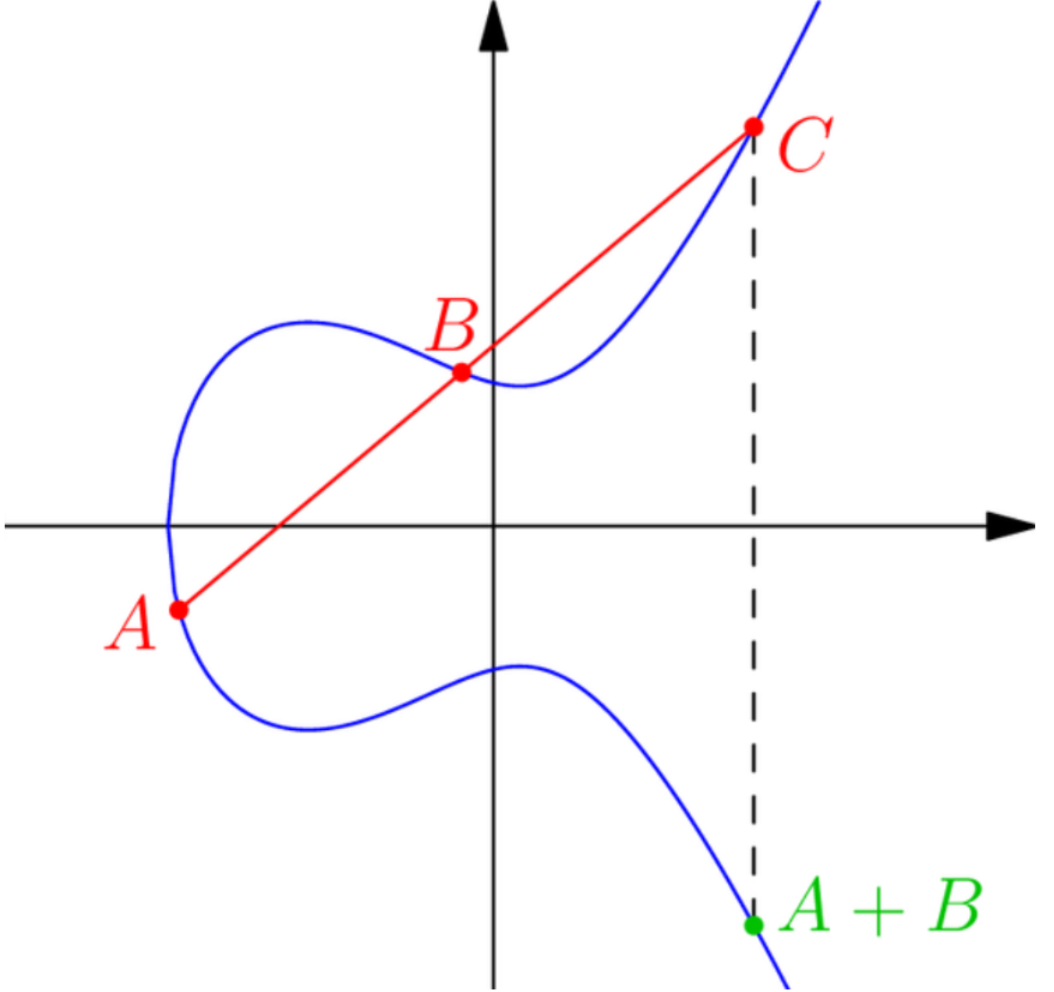
\includegraphics[width=\linewidth]{gfx/elliptic_curves_addition.png}
    \caption{Illustration of addition on elliptic curves}
    \label{fig:ell_curves_add}
\end{wrapfigure}

We define an addition operation for points on the elliptic curve.
The addition can be illustrated as shown in Figure \ref{fig:ell_curves_add}.
When two points $A$ and $B$ are added, first, the line that crosses both points will be found.
This line will cross the curve at another point, which is the point $-A+B$.
If we mirror the point on the x-axis, we get the point $A+B$ i.e the point resulting from the addition operation.

In case both points are the same, the line will be the tangent of the curve.
In case $A$ is added to $-A$, the line would be horizontal, thus not crossing the curve again.
The result of this operation is defined as the point at infinity $\mathcal{O}$.

When calculating with an elliptic curve, the concept is very similar to calculating in $mod$.
We have a generator Point $\mathcal{G}$ on $E$, which we will add to itself to produce new points in $E$.
The discrete logarithm problem on elliptic curves expresses \textit{how many times must $\mathcal{G}$ be added to itself to produce a Point Y?}:
$DLog_{\mathcal{G}}^{E}(Y)$ is the value $x$ for which $x\mathcal{G} = Y$.

If we had a given $Z_p^*$ and we could find an elliptic curve $E$ with the number of distinct elements $q$, such that $q$ is very close to $p$, this would be better than using a prime subgroup of $Z_p^*$.
The reason is that a prime subgroup of $Z_p^*$ would require us to choose $q << p$ because of the attacks shown in Section \ref{sec:index_caclulus} and \ref{sec:sec:number_field_sieve} work against subgroups of $Z_p^*$.
These smaller values are much faster to compute than bigger values.
The question now is whether given $Z_p^*$ it is actually possible to find an elliptic curve with its number of elements close to $p$.
Hasse's theorem shows that it is possible to find an elliptic curve with the number of elements relatively close to $p$ (with "only" up to $2\sqrt{p}$ distance to $p$):

$$
    p+1 - 2 \sqrt{p} \leq \; |E_{a,b}| \leq p+1 + 2 \sqrt{p}\;
$$

In practice, the value for $p$ and the elliptic curve is given.
Those are defined through standards published by e.g. the BSI.

The Youtube channel \url{https://www.youtube.com/@thenativeweb} also explains elliptic curves very nicely in the videos \textit{Architecture's Daily} episodes 91 to 95.

\section{Diffie-Hellman Key Exchange}\label{sec:diffie_hellman}

The Diffie-Hellman key exchange claims a way to generate a common secret key for two communication partners over a public channel.

\begin{figure}[h]
    \center
    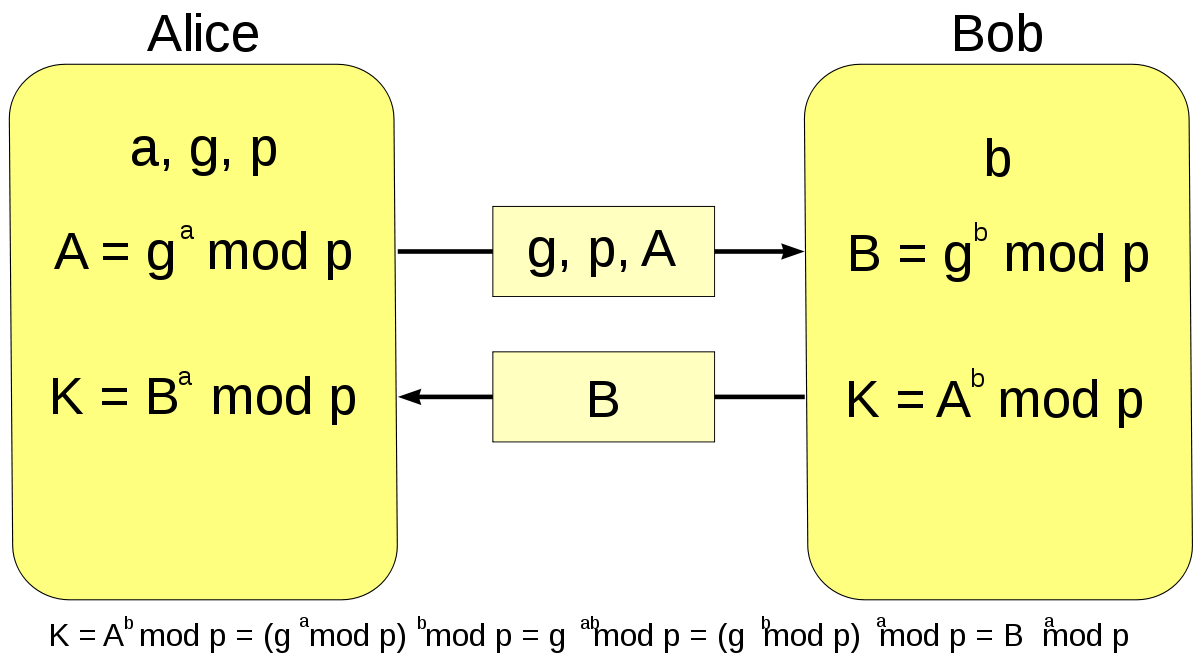
\includegraphics[width=\linewidth]{gfx/diffie-helman.png}
    \caption{Illustration of the Diffie-Hellman key exchange. Note that $g$ and $p$ can be generated by Alice, like shown here, or delivered by a third party (since both values are public).}
    \label{fig:diffie_hellman}
\end{figure}


\section{IND-CPA and IND-CCA for PKE}

IND-CPA and IND-CCA for PKE (public key encryption) are defined the same way as for symmetric encryption:

\begin{figure}[h]
    \center
    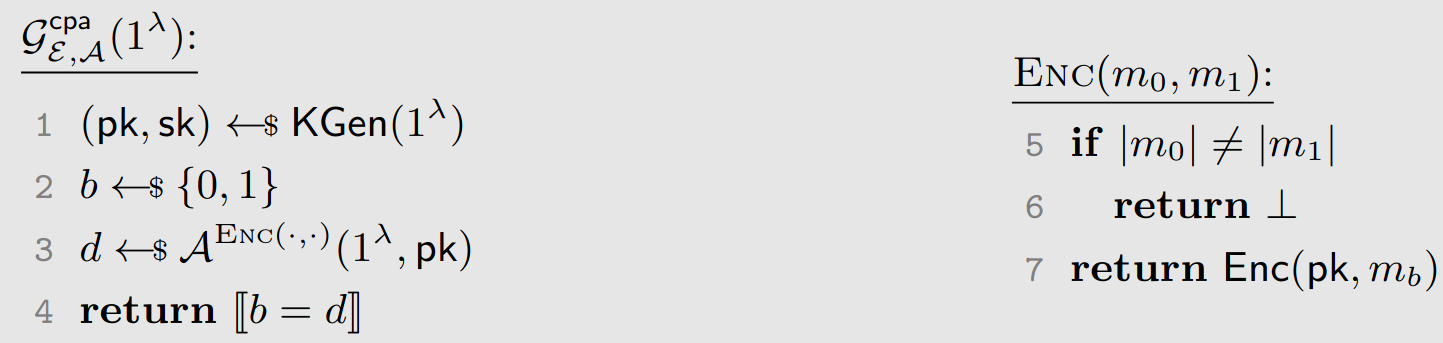
\includegraphics[width=\linewidth]{gfx/IND-CPA_PKE.png}
    \caption{Game-Based definition of IND-CPA for PKE. A PKE system $\epsilon = KGen$, $Enc$, $Dec$ is secure if for all PPT adversaries $A$, there is a negligible function $neg(\lambda)$, such that $Pr[G^{cpa}_{A,\epsilon}(1^\lambda)] = \frac{1}{2} + neg(1^\lambda)$}
    \label{fig:ind-cpa-PKE}
\end{figure}

\begin{figure}[h]
    \center
    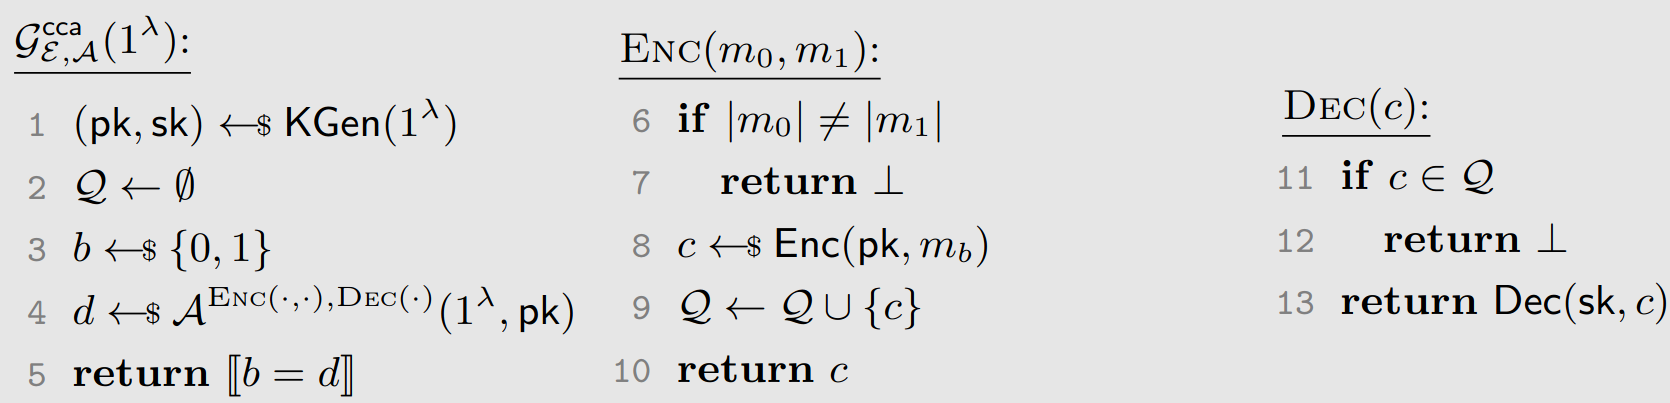
\includegraphics[width=\linewidth]{gfx/IND-CCA_PKE.png}
    \caption{Game-Based definition of IND-CCA for PKE. A PKE system $\epsilon = KGen$, $Enc$, $Dec$ is secure if for all PPT adversaries $A$, there is a negligible function $neg(\lambda)$, such that $Pr[G^{cca}_{A,\epsilon}(1^\lambda)] = \frac{1}{2} + neg(1^\lambda)$}
    \label{fig:ind-cca-PKE}
\end{figure}

There are a couple of things that should be kept in mind when dealing with these definitions in comparison to the symmetric versions:

\begin{enumerate}
    \item For PKE, it does not matter how many times the adversary queries $ENC$. So $IND$ and $IND-CPA$ are equivalent.
    \item An additional $ENC'(m) \rightarrow c$ oracle that only takes one message and encrypts it (without a bit $b$), does not help the adversary, since the adversary can compute ciphertexts itself anyways because the $Enc$ function does not involve a secret key.
    \item Any deterministic algorithm cannot be $IND-CPA$ even if the adversary only queries $ENC$ once (i.e. $IND$), because the adversary can compute ciphertexts itself. If $Enc$ is deterministic, the attacker could query $ENC(m_0, m_1)$ and receive $c_b$. Then he could compute $Enc(pk,m_0) \rightarrow c_0$ itself and compare it with $c_b$.\footnote{Compare section \ref{sec:ind-cpa-sym}}
\end{enumerate}



\section{ElGamal Encryption}\label{sec:elgamal}

\begin{align*}
     & \underline{KGen(1^\lambda):}           &  & \underline{Enc(pk, (G,g,q), m):}   &  & \underline{Dec(sk, (Y,c)):} \\
     & (G,g,q) \leftarrow GroupGen(1^\lambda) &  & y \leftarrow\$ G                   &  & return c \cdot Y^{-sk}      \\
     & sk \leftarrow\$ G                      &  & \text{return } (g^y, pk^y \cdot m) &  &                             \\
     & pk \leftarrow g^{sk} \text{ in } G     &  &                                    &  &                             \\
     & \text{return } ((G,g,q), (sk, pk))     &  &                                    &  &
\end{align*}

ElGamal is IND-CPA if the DDH assumption (see section \ref{fig:DDH_assumption}) holds.
However, it is \emph{not} IND-CCA because it has the following property:

$$
    Dec(sk, (Y, c \cdot r)) = Dec(sk, (Y, c)) \cdot r
$$

This holds because of $Dec(sk, (Y, c \cdot r)) = Y^{-sk} \cdot c \cdot r = g^{-sk \cdot y} \cdot g^{sk \cdot y} \cdot m \cdot r = m \cdot r = Dec(sk, (Y, c)) \cdot r$.
This allows an adversary to modify the ciphertext with a known outcome.
The adversary can then divide $r$ back out.
This way, ciphertexts $c$ can be decrypted without querying $c$ at the $DEC$ oracle, allowing us to compare them with an earlier from $ENC$ obtained $c$, this way breaking IND-CCA.

A further restriction of ElGamal is that all messages must be in the group $G$ and therefore have a certain length and structure.
Both problems are solved by ICIES.

\section{ICIES encryption}\label{sec:ICIES}

% TODO: differentiate between elgamal and DH

The ICIES (Elliptic Curve Integrated Encryption Scheme) encryption is a modern standardized version of the ElGamal encryption concept and uses Diffie-Hellman and the common key $K$ that it generates as the input for a PRF to create a key for symmetric encryption and authentication.

ICIES uses Diffie-Hellman for key exchange to generate two keys $(k_E, k_M)$, one for symmetric encryption and one for key exchange.
It then uses encrypt and MAC, which we have learned earlier.
Additionally, it uses a key derivation function (KDF).
The purpose of this function is simply to transform points on the elliptic curve into a binary representation that can be used as a key.
This means that KDF works like a hashing function.
For simplicity, in the following, we use the notation above $Z_p^*$ although ICIES in reality work with elliptic curves.
The operations of ICIES are formally defined as follows:

\begin{align*}
     & \underline{KeyGen(1^\lambda)}:         &  & \underline{Enc(pk, m)}                 &  & \underline{Dec(sk,(Y,c,\tau))}                              \\
     & (G,g,q) \leftarrow GroupGen(1^\lambda) &  & y             \leftarrow Z_p^*         &  & (k_E,k_M)                            \leftarrow KDF(Y^{sk}) \\
     & sk \leftarrow  G                       &  & Y             \leftarrow g^y           &  & \textit{if } MAC(k_M, c) \;!=\; \tau  \text{ return } \perp \\
     & pk  \leftarrow g^{sk}                  &  & (k_E, k_M)    \leftarrow KDF(pk^y)     &  & \text{return } SymDec(k_E,c)                                \\
     & \text{return } ((G,g,q), (pk,sk))      &  & c             \leftarrow SymEnc(k_E,m) &  &                                                             \\
     &                                        &  & \tau          \leftarrow MAC(k_M,c)    &  &                                                             \\
     &                                        &  & \text{return }(Y,c,\tau)               &  &                                                             \\
\end{align*}

$KeyGen$ is executed on the receiver side.
Then the public key must be published.
Afterwards, $Enc$ can be executed by senders.
The receiver can then decrypt the ciphertexts $(Y, c, \tau$) using $Dec$.

This is a so-called KEM-DEM hybrid encryption.
\textit{KEM (Key Encapsulation)} refers to a process of not explicitly encrypting the key as one arbitrary message (in contrast to asynchronous encryption), but instead, only encrypting a key. Because optimizations can be applied, this can be faster than asynchronous encryption.
\textit{DEM (Data Encapsulation)} refers to using a symmetric key for encrypting data.
\textit{KEM-DEM Hybrid} describes using an asymmetric KEM system for generating a key and a faster symmetric DEM system for encrypting payload data.

KEM-DEM hybrid encryption combines the simple key management of asynchronous encryption with the high performance of synchronous encryption.
On the other hand, we need two systems instead of one, an asynchronous one and a synchronous one.

ICIES is IND-CCA if a DH-like assumption holds and if the symmetric encryption used is IND-CPA and the MAC used is sEUF-CMA.

\section{Discrete Security Assumptions}

This chapter will explain the discrete security assumptions DL, CDH and DDH.
It can be proven that if DDH holds, CDH must hold and if CDH holds, DL must hold.
But we do not know the reverse.
All these assumptions are unbroken for more than 40 years know, however, not been proven either.

\subsection{DL (Discrete Logarithm) Assumption}

\begin{wrapfigure}{r}{0.4\textwidth}
    \center
    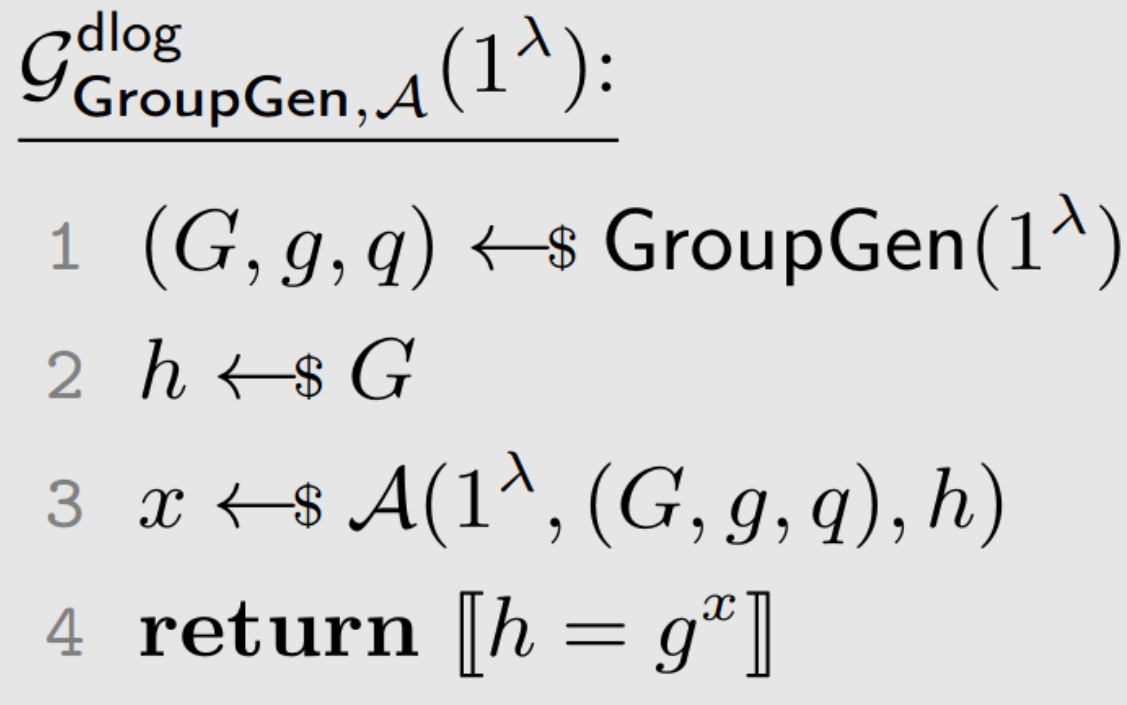
\includegraphics[width=\linewidth]{gfx/discrete_log_assumption.png}
    \caption{Game-based definition of the DL assumption.}
    \label{fig:DL_assumption}
\end{wrapfigure}

The discrete logarithm assumption is that given a group $(G,g,p)$ and a value $y \in G$, the discrete logarithm $DLog_g(y)$ is not efficiently computable.
This can be defined through the game shown in Figure \ref{fig:DDH_assumption}.
DL then states the following regarding the game for all $PPT$ adversaries $A$:

$$
    Pr[Exp_{GroupGen,A}^{dlog}(1^\lambda) = 1] \leq neg(\lambda)
$$


\subsection{CDH (Computational Diffie-Hellman) Assumption}

\begin{wrapfigure}{r}{0.4\textwidth}
    \center
    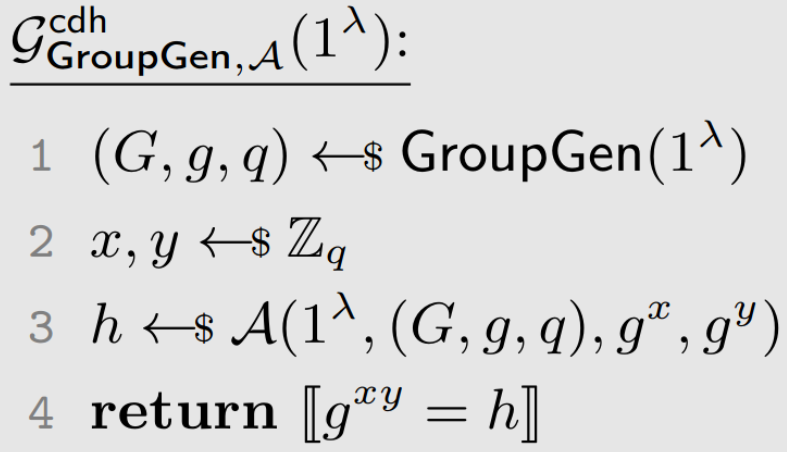
\includegraphics[width=\linewidth]{gfx/CDH_assumption.png}
    \caption{Game-based definition of the CDH assumption.}
    \label{fig:CDH_assumption}
\end{wrapfigure}


The computational Diffie-Hellman assumption states that given a group $(G,g,p)$ and two values $g^x$ and $g^y$, $g^{xy}$ cannot be computed efficiently (of course without knowing $x$ and $y$ but only knowing the powers).
If this holds, DL must also hold (can be shown by reduction).
This can be defined through the game shown in Figure \ref{fig:DDH_assumption}.
CDH then states the following regarding the game for all $PPT$ adversaries $A$:

$$
    Pr[Exp_{GroupGen,A}^{cdh}(1^\lambda) = 1] \leq neg(\lambda)
$$


\subsection{DDH (Decisional Diffie-Hellman) Assumption}

\begin{wrapfigure}{r}{0.4\textwidth}
    \center
    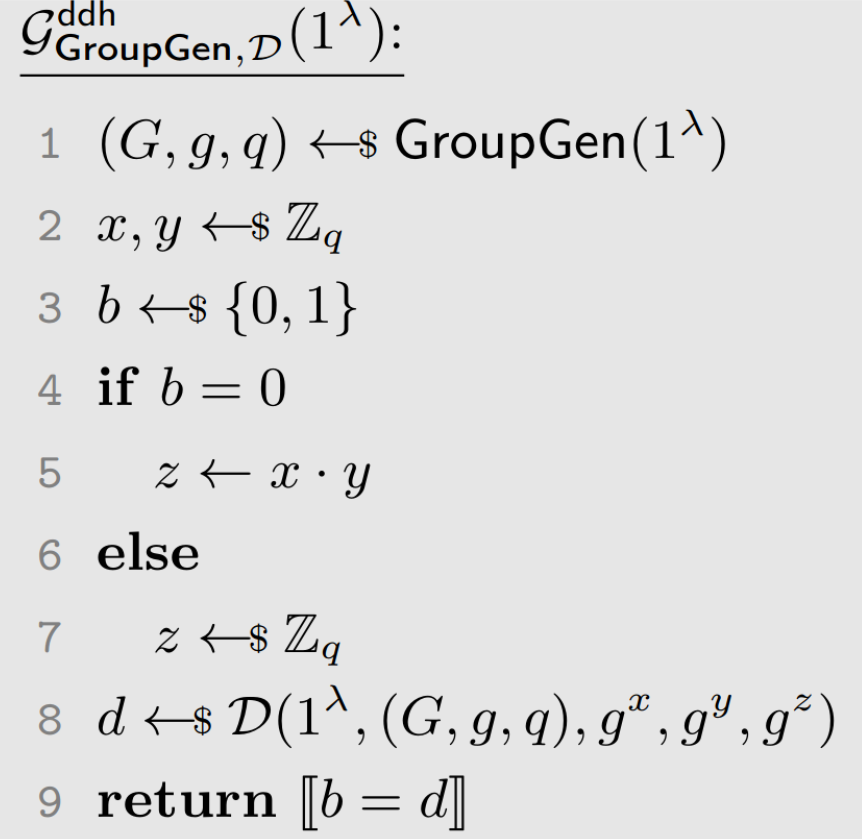
\includegraphics[width=\linewidth]{gfx/DDH_assumption.png}
    \caption{Game-based definition of the DDH assumption.}
    \label{fig:DDH_assumption}
\end{wrapfigure}

The decisional Diffie-Hellman assumption states that given $(G,p,g)$, $g^x$ and $g^y$, the two values $g^{xy}$ and $g^z$ can not be distinguished efficiently.
If this holds, CDH must also hold (can be shown by reduction).
This can be defined through the game shown in Figure \ref{fig:DDH_assumption}.
DDH then states the following regarding the game for all $PPT$ adversaries $A$:

$$
    Pr[Exp_{GroupGen,}^{ddh}(1^\lambda) = 1] \leq \frac{1}{2} + neg(\lambda)
$$


\section{Textbook-RSA}\label{sec:textbook_rsa}


\begin{align*}
     & \underline{KeyGen(1^\lambda)}:         &  & \underline{Enc((N,e), m)} &  & \underline{Dec((N,d), c)} \\
     & (N, e, d) \leftarrow RSAGen(1^\lambda) &  & \text{return }(m^e mod N) &  & \text{return } c^d mod N  \\
     & \text{return } (N, e, d)               &  &                           &  &                           \\
\end{align*}

The correctness is assured because $RSAGen$ chooses two prime numbers $p$ and $q$ (of similar lengths) to compute $N$.
Because we know that $\Phi(p \cdot q) = (p-1)(q-1)$, the algorithm can compute an exponent $e$ that has a multiplicative inverse in $mod\; \Phi(N)$ (fulfilled if $gcd(e, \Phi(N)) = 1)$.
Then the $RSAGen$ algorithm can also compute that inverse $d$ of $e$ for which $d \cdot e = 1 \;mod\; \Phi(N)$ since it knows $\Phi(N)$.
Because we know that $\forall x \in Z_m^* :\; x^r = x^{r \;mod\; \Phi(m)} \;mod\; m $ the correctness of Textbook RSA follows as:

\begin{align*}
    m & = Dec((N,d), Enc((N,e), m))               \\
      & = Dec((N,d), m^d \;mod\; N)               \\
      & = m^{d \cdot e} \;mod\; N                 \\
      & = m^{d \cdot e \;mod\; \Phi(N) \;mod\; N} \\
      & = m^1 \;mod\; N                           \\
      & = m
\end{align*}

Textbook-RSA is not IND-CPA and therefore also not IND-CCA because it is a deterministic encryption system (see Section \ref{sec:ind-cpa-sym}).

Furthermore, another property of Textbook-RSA interferes with IND-CCA.
Textbook-RSA has a \emph{homomorphism} property (just like ElGamal).
This means that $Enc(m_0) \cdot Enc(m_1) = Enc(m_0 \cdot m_1)$ because $Enc(m_0) \cdot Enc(m_1) = m_0^e \;mod\;N\; \cdot m_1^e \;mod\;N\; = (m_0 * m_1)^e \;mod\;N = Enc(m_0 \cdot m_1)$.
Using this, an adversary against IND-CCA can query $ENC(m_0, m_1) \rightarrow c_b$ and then query $DEC(c_b \cdot c_b) \rightarrow m^*$ (because $c_b \cdot c_b$ has never been returned by $ENC$ before).
Then he could compare $m^*$ with $m_0 \cdot m_0$ or with $m_1 \cdot m_1$ to find out $b$.

RSA is also called a \emph{trapdoor function}, because it is not invertible if $d$ is unknown, but if $d$ is known (or something that gets us to $d$ e.g. $p$ and $q$), it is invertible (trapdoor opened by $d$).

\section{RSA assumption}

RSA is based on the RSA assumption defined through the following security game $Exp^{RSA}{A}$:

\begin{align*}
    \underline{Exp^{RSA}(1^\lambda):} &                                  \\
    (N,e,d)                           & \leftarrow\$ \;RSAGen(1^\lambda) \\
    x                                 & \leftarrow\$ \;Z_N^*             \\
    y                                 & \leftarrow x^e \; mod \; N       \\
    x*                                & \leftarrow A(1^\lambda, N, e, y) \\
    return                            & \; [(x^*)^e = y \; mod \; N]
\end{align*}

For all PPT algorithms $A$ there exists a negligible function $neg(\lambda)$ such that:

$$
    Pr[Exp^{RSA}(1^\lambda) = 1] \leq neg(\lambda)
$$

In other words, there is no efficient algorithm that can compute the message $x$ or an equivalent value without knowledge of $d$.

This assumption is tightly coupled with the assumption that it is difficult to factorize prime number products:
Given a product of prime numbers $N = p \cdot q$, we assume there is no efficient algorithm that computes $p$ and $q$.
If this does not hold, an adversary to RSA could factorize $N$ to $p$ and $q$ and then compute $Phi(N)$ as $(p-1) \cdot (q-1)$ and from that $d$ in the same way that the $RSAGen$ algorithm does.

So we know if the RSA assumption holds, then prime factorization must also be difficult.
However, if prime factorization is difficult, we do not know if the RSA assumption holds because there might be another way of breaking RSA that we do not know yet.


\section{Optimal Asymmetric Encryption Padding (OAEP)}\label{sec:oaep}

\begin{wrapfigure}{r}{0.5\textwidth}
    \center
    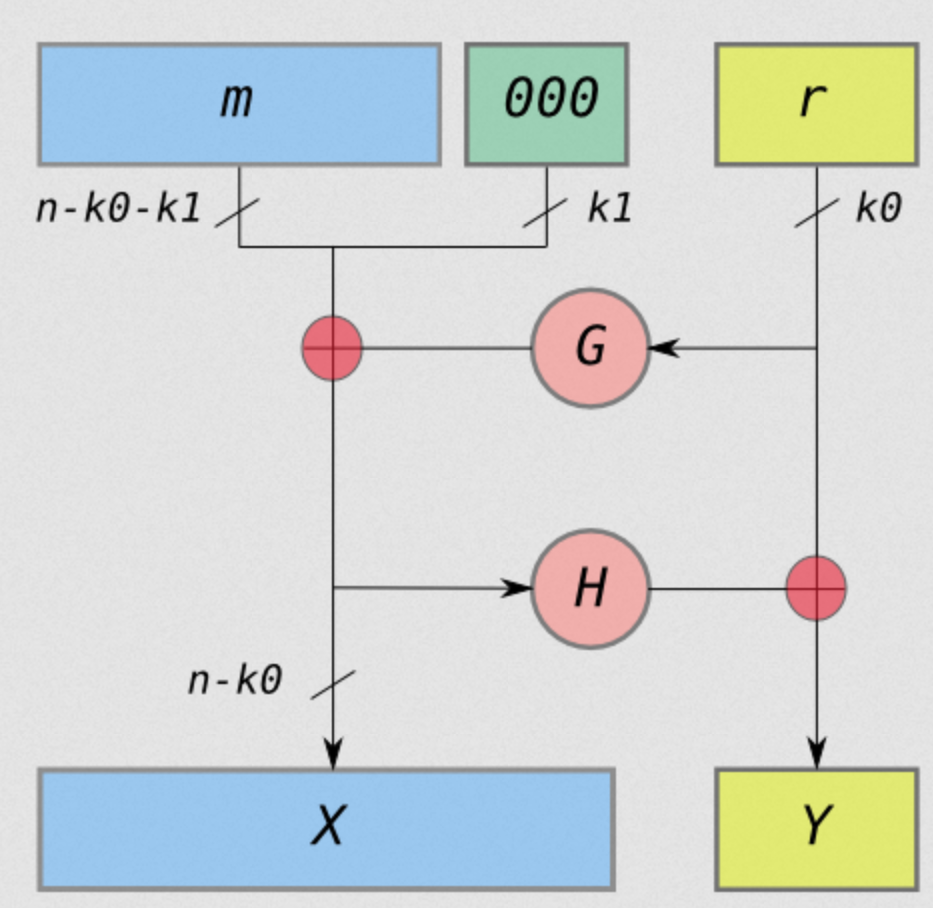
\includegraphics[width=\linewidth]{gfx/OAEP.png}
    \caption{OAEP permutation before applying RSA function}
    \label{fig:OAEP}
\end{wrapfigure}

To build an IND-CCA secure encryption system utilizing the RSA function that does not have the drawbacks of textbook RSA (determinism, homomorphism), the OAEP system has been developed.
It adds two different types of padding to the message and uses two hash functions $G$ and $H$ to combine the messages.
Afterwards, the resulting new bit string $X||Y$ is used as input for the RSA function.

The first type of padding is a random part $r$ consisting of $k_0$ bits.
This adds the probabilistic component to the encryption, therefore making it IND-CPA:
Since $G$ produces random bits based on $r$, the left side becomes a pseudo-random string.
Afterwards, we use this as input for $H$ and add the resulting pseudo-random string to the right part.
Therefore, both, $X$ and $Y$ will look like random bit strings.
Using then RSA on top of that makes it IND-CPA (full proof not discussed here.)

The second type of padding is a field of $k_0$ zero-bits.
These are used for checking the integrity of decrypted ciphertexts and thereby ensuring IND-CCA:
When decrypting a ciphertext, the $Dec$ function first computes the inverse of the RSA function using $d$, thereby reconstructing $X||Y$.
Then the Feistel network is traversed from the bottom up (hash functions do not need to be inverted, they will cancel out by XOR).
If an adversary tries to modify a ciphertext $c$ before passing it to $DEC$, the zero-bits will be modified (contain ones) with high probability due to the diffusion done by the Feistel.
In this case, $Dec$ will return an error, thereby preventing adversaries from modifying and then decrypting ciphertexts.
This way, the IND-CCA attack against textbook RSA, which was based on the homomorphism of the RSA function, is no longer possible.

\chapter{Glossary}

In this chapter, basic terms will be defined and explained.

\section{Kerckhoffs's Principle}

Security should not require the system, but merely the key to be secret.

\section{Perfect Security}

A cryptographic process is perfectly secure if for all messages in the set of possibles messages $m \in M$ and all possibly producible ciphertexts $c \in C \quad|\quad Pr[C=c] > 0$ the probability that $m$ occurs is equal no matter if the ciphertext is known or unknown: $Pr[M=m] = Pr[M=m | C=c]$. More simply put, this means that an attacker cannot gain any knowledge about the message when seeing its ciphertext regardless of the message's and the ciphertext's concrete values.

\section{Conditional Probability}

Conditional probability $Pr[A=a | B=b]$ is the probability that the event $a \in A$ occurs if it is already known that the event $b \in B$ occurs. It is calculated as $Pr[A=a | B=b] = \frac{Pr[A=a] \wedge Pr[B=b]]}{Pr[B=b]}$. An example is a probability rolling a 6-sided dice results in the number 6 if it is already known that the result is an even number: $Pr[is 6 | is even] = \frac{Pr[is 6] \wedge Pr[is even]}{is even} = \frac{\frac{1}{6}}{\frac{1}{2}} = \frac{1}{3}$.

Perfect security can only be reached for processes with deterministic a decryption function if the key space is at least as big as the message space $|K| \geq |M|$. This is because then a given ciphtertext $c$ could be decrypted to $|K|$ different messages $m$ (determinism), which minimizes the search space for an attacker from $|M|$ possibilities to $|K|$ possibilities and therefore also decrease the attacker's uncertainty..

\section{Hiding Message Length}

Completely hiding the length of a message is impossible if the length of possible messages is unlimited. Hiding messages' lengths would require changing their length for transmission. The message length cannot be decreased because this would result in data loss. Therefore, messages would have to be extended up to at least the size of the longest possible message to make all messages appear to have the same length. If the message size is unlimited, we cannot expand messages to that nonexisting limit.

\section{Insecurity of Shift-Ciphers}

Shift-ciphers, like Ceasar, are not perfectly secure, which can be shown by contraposition: If the possible messages are defined as $M=\{aa, ab\}$, a shift cipher shifting each character by some number of characters in an alphabet would always create ciphertexts as follows $Dec(aa) \rightarrow c_{0}c{0}$ and $Dec(ab) \rightarrow c_{0}c_{1} \quad|\quad c_{0} \neq c_{1}$ Therefore, an attacker's probability when seeing the ciphertexts to guess the correct message $m \in M$ is equal to $1$ and greater than the initial probability, which was $\frac{1}{2}$. A concrete example would be: $Pr[M=aa | C=c_{0}c_{0}] = 1 \neq Pr[M=aa] = \frac{1}{2}$. We see that limiting the set of possible messages can be a helpful method for contradictions of perfect correctness.

%*************************************************************************
% Recommendations
%*************************************************************************
%\part{Empfehlungen zur Erstellung wissenschaftlicher Abschlussarbeiten}
%\label{pt:recommendations}
%*************************************************************************
% Backmatter
%*************************************************************************
% \appendix
%\renewcommand{\thechapter}{\alph{chapter}}
% \cleardoublepage
% \part{Appendix}
%*************************************************************************
% Other Stuff in the Back
%*************************************************************************
\cleardoublepage%********************************************************************
% Bibliography
%*******************************************************
% work-around to have small caps also here in the headline
% https://tex.stackexchange.com/questions/188126/wrong-header-in-bibliography-classicthesis
% Thanks to Enrico Gregorio
% \defbibheading{bibintoc}[\bibname]{%
%   \phantomsection
%   \manualmark
%   \markboth{\spacedlowsmallcaps{#1}}{\spacedlowsmallcaps{#1}}%
%   \addtocontents{toc}{\protect\vspace{\beforebibskip}}%
%   \addcontentsline{toc}{chapter}{\tocEntry{#1}}%
%   \chapter*{#1}%
% } 
\printbibliography[heading=bibintoc]

%*************************************************************************
% Game Over: Restore, Restart, or Quit?
%*************************************************************************
\end{document}
%*************************************************************************

% NOTE: COMPILATION HANGS SOMETIMES, IF WE HAVE A pages ATTRIBUTE IN THE BIBLIOGRAPHY. I DO NOT KNOW WHY

